% !TEX program = xelatex
% 策联杯 A 题：锂离子电池快充策略对寿命衰减的影响建模与优化
\documentclass[withoutpreface]{cumcmthesis}

\usepackage[framemethod=TikZ]{mdframed}
\usepackage{url}
\usepackage{subcaption}
\usepackage{geometry}
\usepackage{setspace}
\usepackage{array}
\usepackage{graphicx}
\usepackage{multirow}
\usepackage{hyperref}
\usepackage{amsmath,amssymb,bm}
\usepackage{float}
\usepackage{placeins}
\usepackage{longtable}
\usepackage{booktabs}
\usepackage{listings,xcolor}
\graphicspath{{figures/}}

\geometry{a4paper,left=25mm,right=25mm,top=25mm,bottom=25mm}
\setlength{\emergencystretch}{2em}

% 代码块样式
\lstdefinestyle{pythonappendix}{
    language=Python,
    basicstyle=\ttfamily\scriptsize,
    keywordstyle=\color{blue!55!black},
    commentstyle=\color{green!35!black},
    stringstyle=\color{red!45!black},
    numbers=left, numberstyle=\tiny\color{gray},
    frame=single, breaklines=true,
    columns=fullflexible, tabsize=4,
}
\lstset{style=pythonappendix}

\title{锂离子电池快充策略对寿命衰减的影响建模与优化}

\begin{document}

\maketitle

\begin{abstract}
快充策略在缩短锂离子电池补能时间的同时会加速容量衰减，如何刻画快充策略与寿命衰减的定量关系并兼顾二者优化，是新能源汽车与储能系统的关键问题。本文基于 MIT--Stanford 锂离子电池循环老化数据集（49 块电池、9350 条循环记录、9 种两阶段快充策略），围绕快充策略参数（$C_1$、$Q_1$、$C_2$）对寿命衰减的影响，建立了数据清洗、统计推断、寿命预测到多目标优化的完整流程，始终坚持可复现、留出验证与不确定性量化。

\textbf{针对问题一：} 完成最小干预的数据清洗（修复 3 处异常），以函数型岭回归为主模型、样条混合与多项式混合为候选，按整块电池留一验证估计各策略 SOH 曲线。三种模型的策略排序完全一致，主模型 LOBO RMSE 为 $0.004338$；典型长寿命策略为 $3\_6C$--$80PER\_3\_6C$ 与 $5C\_67PER\_4C$，短寿命为 $3\_7C\_31PER\_5\_9C$ 与 $80PER\_3\_6C$，但置换检验与 Holm 校正后两两间无显著差异。

\textbf{针对问题二：} 引入低维应力坐标（总电流应力 $J$ 与高 SOC 加权应力 $H$）建立约束退化混合模型。全局置换检验显示策略间末段退化率差异显著（$p=5\times10^{-5}$），但选择校正后 $p=0.065$，且删除极端策略后常数模型胜出——9 种策略的稀疏混杂设计不足以识别三个参数的独立因果效应，本文如实报告该边界。

\textbf{针对问题三：} 经嵌套留一验证冻结轨迹岭回归模型 $C\_ridge$，其 $L=150$ 策略等权 LOBO RMSE 为 $0.000660$；给出 9 块测试电池 151--200 循环预测与保守点区间，80\% 寿命仅作情景外推（691.6--3653.0 循环）。

\textbf{针对问题四：} 采用观测策略离散 Pareto 与整块电池 bootstrap。若优先缩短时间并接受约 0.17\% 退化，推荐 \textbf{$5\_3C\_54PER\_4C$（$C_1=5.3,Q_1=54\%,C_2=4.0$）}：较长寿命策略缩短约 25\% 时间、退化仅增约 0.12 个百分点。连续参数响应面因 oracle 压力测试失败被淘汰。

跨问题一致结论：充电策略标签与 SOH 退化相关，早期 SOH 动态是短期预测的主要信息，但稀疏混杂设计使结论须限制在已观测策略内，所有寿命终点均为外推估计。

\keywords{\textbf{锂离子电池\quad 快充策略\quad 函数型岭回归\quad 混合效应模型\quad 留一验证\quad Pareto 优化}}
\end{abstract}

\section{问题重述}
\subsection{问题背景}
锂离子电池的快速充电能够显著缩短补能时间、提高使用便利性，但过高的充电电流会导致电池内部极化增强、热效应加剧与副反应加速，从而加快容量衰减、缩短电池寿命\upcite{keil2016charging}。电池寿命通常以健康状态 SOH 表征，定义为当前可用容量与初始容量之比，本题统一以 80\% SOH 作为寿命终止阈值。

影响电池寿命的两个主要指标为充电倍率（C-rate）与荷电状态 SOC。不同 SOC 区间内电池对充电电流的敏感程度不同：在低 SOC 区间采用较大电流可能有助于缩短充电时间，而在中高 SOC 区间继续采用高倍率充电则可能加剧老化。本题采用 MIT--Stanford 公开数据集（49 块 A123 18650 磷酸铁锂电池，额定容量 1.1 Ah），各电池放电策略一致，差异体现在两阶段快充策略：先以 $C_1$ 倍率从 0\% 充电至 $Q_1$，再以 $C_2$ 倍率从 $Q_1$ 充电至 80\%，最后以 1C 恒流--恒压（CC--CV）充至满电。

\subsection{问题要求}
\begin{itemize}
\item [(1)] 整理数据，分析不同快充策略下的寿命分布，提取并对比典型长寿命与短寿命策略；
\item [(2)] 分析充电策略参数（$C_1,Q_1,C_2$）对寿命衰减的影响，检验差异显著性及参数影响程度；
\item [(3)] 基于 9 块测试电池截至第 150 循环的数据建立寿命预测模型，预测第 151--200 循环 SOH 并外推寿命，评价精度及早期数据长度的影响；
\item [(4)] 设计兼顾充电时间与寿命衰减的策略优化方法，给出推荐策略并与典型策略对比。
\end{itemize}

\section{问题分析}
\subsection{数据特点}
本数据集有三个关键特征：\textbf{（1）}9350 条循环记录是 49 块电池的重复测量，观测非独立，显著性检验与交叉验证必须按整块电池划分；\textbf{（2）}仅有 9 种策略，$C_1,Q_1,C_2$ 联合变化，参数坐标高度相关，且存在新旧结构/数据批次混杂；\textbf{（3）}数据只观测至第 200 循环，SOH 最低约 0.95，\textbf{无任何电池达到 80\% 终点}，因此寿命终点只能外推\upcite{severson2019data}。

\subsection{各问题分析}
\textbf{问题一}是探索性建模。用函数型/混合效应模型估计各策略 SOH 曲线，按整块电池留一验证选模，以 bootstrap 量化不确定性，识别典型长/短寿命策略。

\textbf{问题二}是统计推断。核心难点是稀疏混杂设计下参数效应不可识别。思路是构造物理启发的低维应力坐标，用约束退化混合模型刻画退化，用置换检验与选择校正检验给出稳健的显著性结论\upcite{saxena2019accelerated,keil2016charging}。

\textbf{问题三}是预测。从早期循环提取轨迹特征，比较六类模型，用嵌套留一验证选择并冻结主模型，预测测试电池未来轨迹并给出区间；寿命终点作为情景外推\upcite{richardson2017gaussian,geslin2023features}。

\textbf{问题四}是优化。在 9 个观测策略上做离散 Pareto 分析，用整块电池 bootstrap 评估前沿稳定性，给出条件约束下的推荐；连续参数搜索因设计不足被谨慎淘汰\upcite{attia2020closed,jiang2021bayesian}。

\section{模型假设}
\begin{itemize}
\item [(1)] 假设电池容量测量误差为随机噪声，单次异常尖峰不代表真实寿命改善，可作为数据质量异常修复；
\item [(2)] 假设各电池放电策略一致，电池间差异来源于充电策略与个体制造差异；
\item [(3)] 假设 SOH 在观测窗口内近似平滑，可用函数型/混合效应模型描述，且平均 SOH 随循环单调下降；
\item [(4)] 假设充电时间主要由两阶段恒流决定，恒压尾段与结构/批次影响作为经验项；
\item [(5)] 假设推断单位是整块电池而非循环记录，显著性检验与重采样均按电池/策略聚类；
\item [(6)] 忽略温度、内阻的精细机理，仅将其作为观测协变量\upcite{liu2019modified}。
\end{itemize}

\section{符号说明}
\begin{longtable}{cc}
	\caption{符号说明}\label{tab:symbols} \\
	\toprule[1.5pt]
	符号 & 含义\\
	\midrule[1pt]
	$C_1$ & 第一阶段充电倍率（低 SOC 区，$0\sim Q_1$）\\
	$Q_1$，$q$ & 阶段切换 SOC（\%）；$q=Q_1/100$\\
	$C_2$ & 第二阶段充电倍率（中高 SOC 区，$Q_1\sim80\%$）\\
	$J$ & 总电流应力 $qC_1+(0.8-q)C_2$\\
	$H$ & 高 SOC 加权应力 $\frac12[C_1q^2+C_2(0.8^2-q^2)]$\\
	$T_0$ & 理想恒流充电时间（min）\\
		$J_{\mathrm{high},s_0}$ & SOC 高于 $s_0$ 区间的倍率应力\\
		$L$ & 早期观测数据长度（循环数）\\
		$b_i$ & 第 $i$ 块电池的基线容量\\
	$\mathrm{SOH}_{i,t}$ & 第 $i$ 块电池第 $t$ 循环的健康状态\\
	$r_i$ & 第 $i$ 块电池的退化率（对数尺度）\\
	$D_p$ & 策略 $p$ 的 200 循环退化量\\
	$T_p$ & 策略 $p$ 的平均充电时间\\
	\bottomrule[1.5pt]
\end{longtable}

\section{数据预处理}
\subsection{原始数据核对}
原始数据含电池级摘要表（49 行）与循环级时序表（9350 行）。核对确认 40 块完整电池包含第 1--200 循环，9 块测试电池（$prediction\_test=1$）仅含第 1--150 循环；共 9 种充电策略。

\subsection{异常识别与可审计修复}
对循环数据逐电池检测局部异常：容量采用 $\pm5$ 循环邻域的稳健 z 分数与相对偏差判定，内阻以 $IR\le0$ 判定为物理无效。修复采用相邻有效循环线性插值，共 3 处（表 \ref{tab:clean}），原始值与修复标记全部保留。

\begin{table}[H]\centering
\caption{数据清洗修复记录}\label{tab:clean}
\begin{tabular}{cccccc}
\toprule
电池 & 循环 & 变量 & 原始值 & 修复值 & 依据\\
\midrule
1 & 12 & 容量/Ah & 1.539054 & 1.074304 & 稳健 z 与相对偏差双超限\\
2 & 12 & 内阻/$\Omega$ & 0 & 0.016869 & 内阻必须为正\\
3 & 12 & 内阻/$\Omega$ & 0 & 0.016683 & 内阻必须为正\\
\bottomrule
\end{tabular}
\end{table}

\begin{figure}[H]\centering
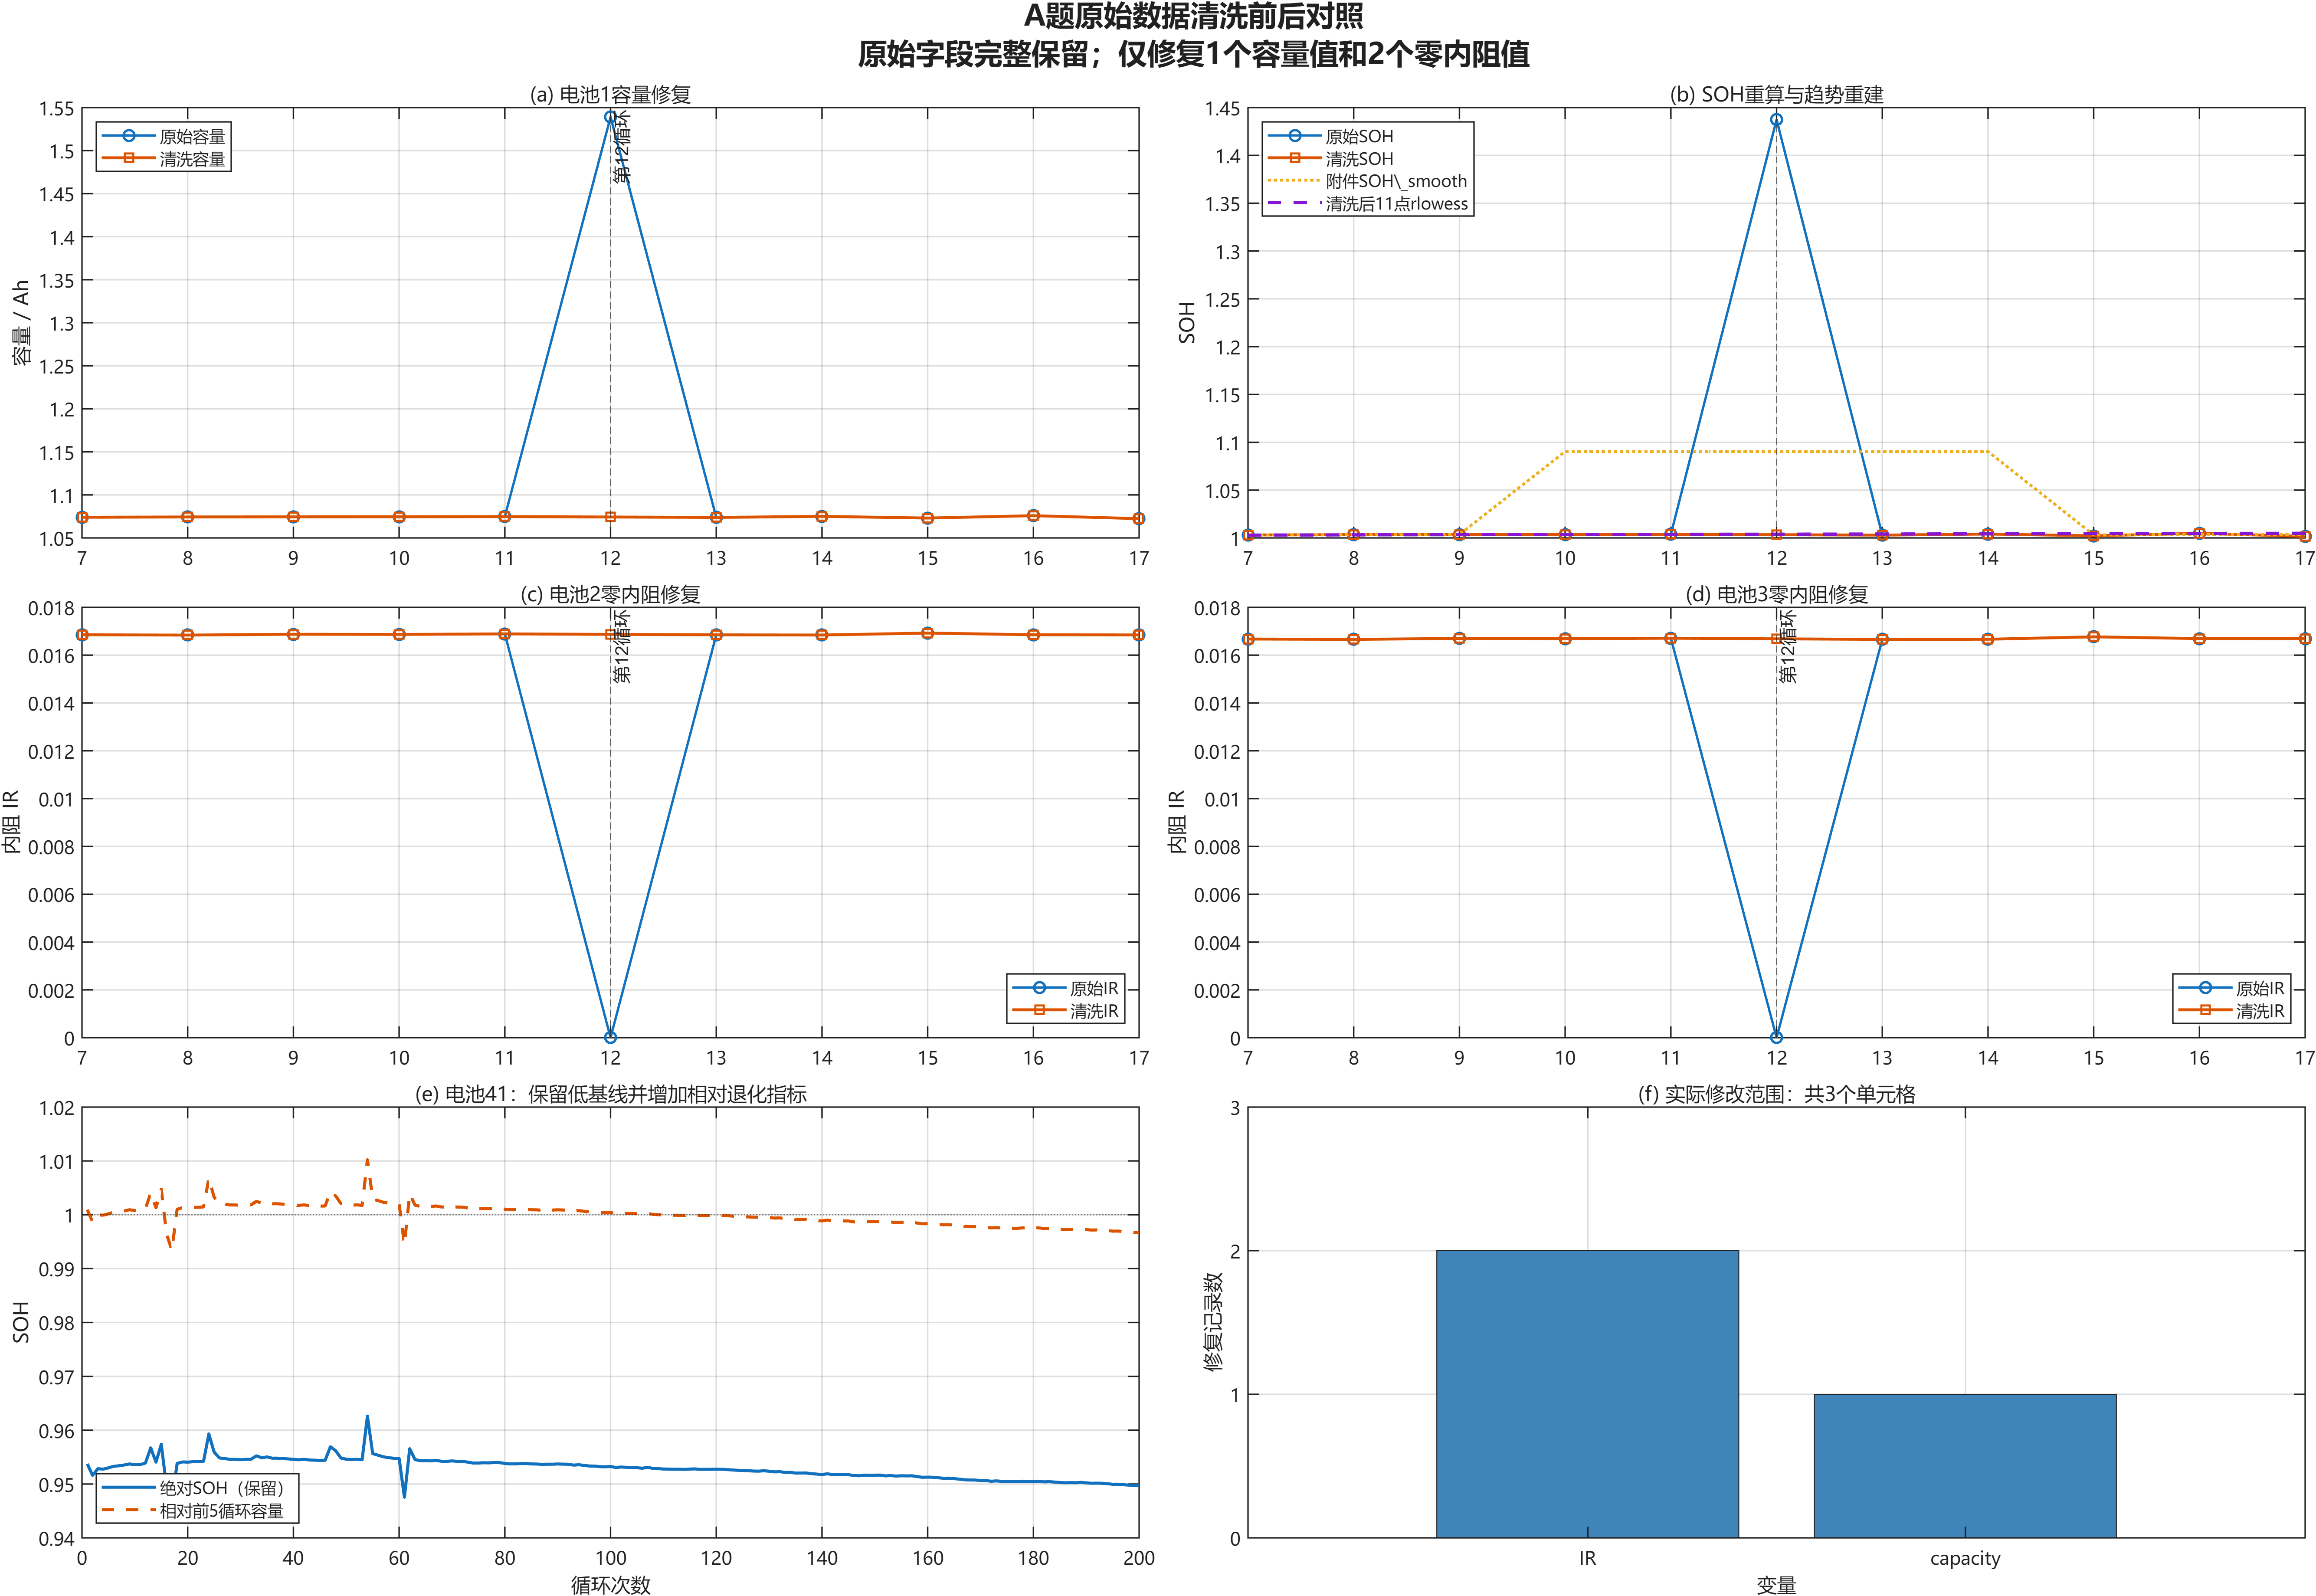
\includegraphics[width=0.95\textwidth]{fig02_cleaning_before_after.png}
\caption{数据清洗前后对照（容量尖峰与零内阻修复）}\label{fig:clean}
\end{figure}

电池 41 存在初始 SOH 基线偏低（约 0.953），判断为批次/定义差异而非单点异常，予以保留并增加相对 SOH 辅助指标；策略 $80PER\_3\_6C$ 的 $C_1$ 缺失（单阶段策略），不猜测填补，仅进入类别比较。清洗后保留全部 49 块电池、9350 条记录。

\section{问题一模型的建立与求解}
\subsection{函数型混合模型}
将每块电池的 SOH 视为关于循环数的函数曲线，建立函数型岭回归主模型
\begin{equation}
\mathrm{SOH}_{i,t}=f(t)+f_{p(i)}(t)+b_i+\varepsilon_{i,t},
\end{equation}
其中 $f(t)$ 为总体非线性退化趋势，$f_{p(i)}(t)$ 为策略 $p(i)$ 的偏离，$b_i$ 为电池个体差异，$\varepsilon_{i,t}$ 为噪声。以样条混合（spline\_mixed）与多项式混合（polynomial\_mixed）为候选对照。模型用 40 块完整电池按整块电池留一验证（LOBO）评价，策略级指标以整块电池 bootstrap 估计标准误与 95\% 区间。

\subsection{模型选择}
三个候选模型的 LOBO RMSE 极其接近（表 \ref{tab:q1_model}），函数型岭以 $0.004338$ 略优，选为主模型；且三模型对第 200 循环 SOH 的策略排序完全一致，说明排序稳健。

\begin{table}[H]\centering
\caption{问题一候选模型比较（LOBO）}\label{tab:q1_model}
\begin{tabular}{lcccl}
\toprule
模型 & 平均电池 RMSE & 平均电池 MAE & 最差策略 RMSE & 选定\\
\midrule
polynomial\_mixed & 0.004394 & 0.004071 & 0.018335 & 否\\
spline\_mixed & 0.004342 & 0.004036 & 0.018332 & 否\\
functional\_ridge & \textbf{0.004338} & 0.004033 & 0.018332 & \textbf{是}\\
\bottomrule
\end{tabular}
\end{table}

\begin{figure}[H]\centering
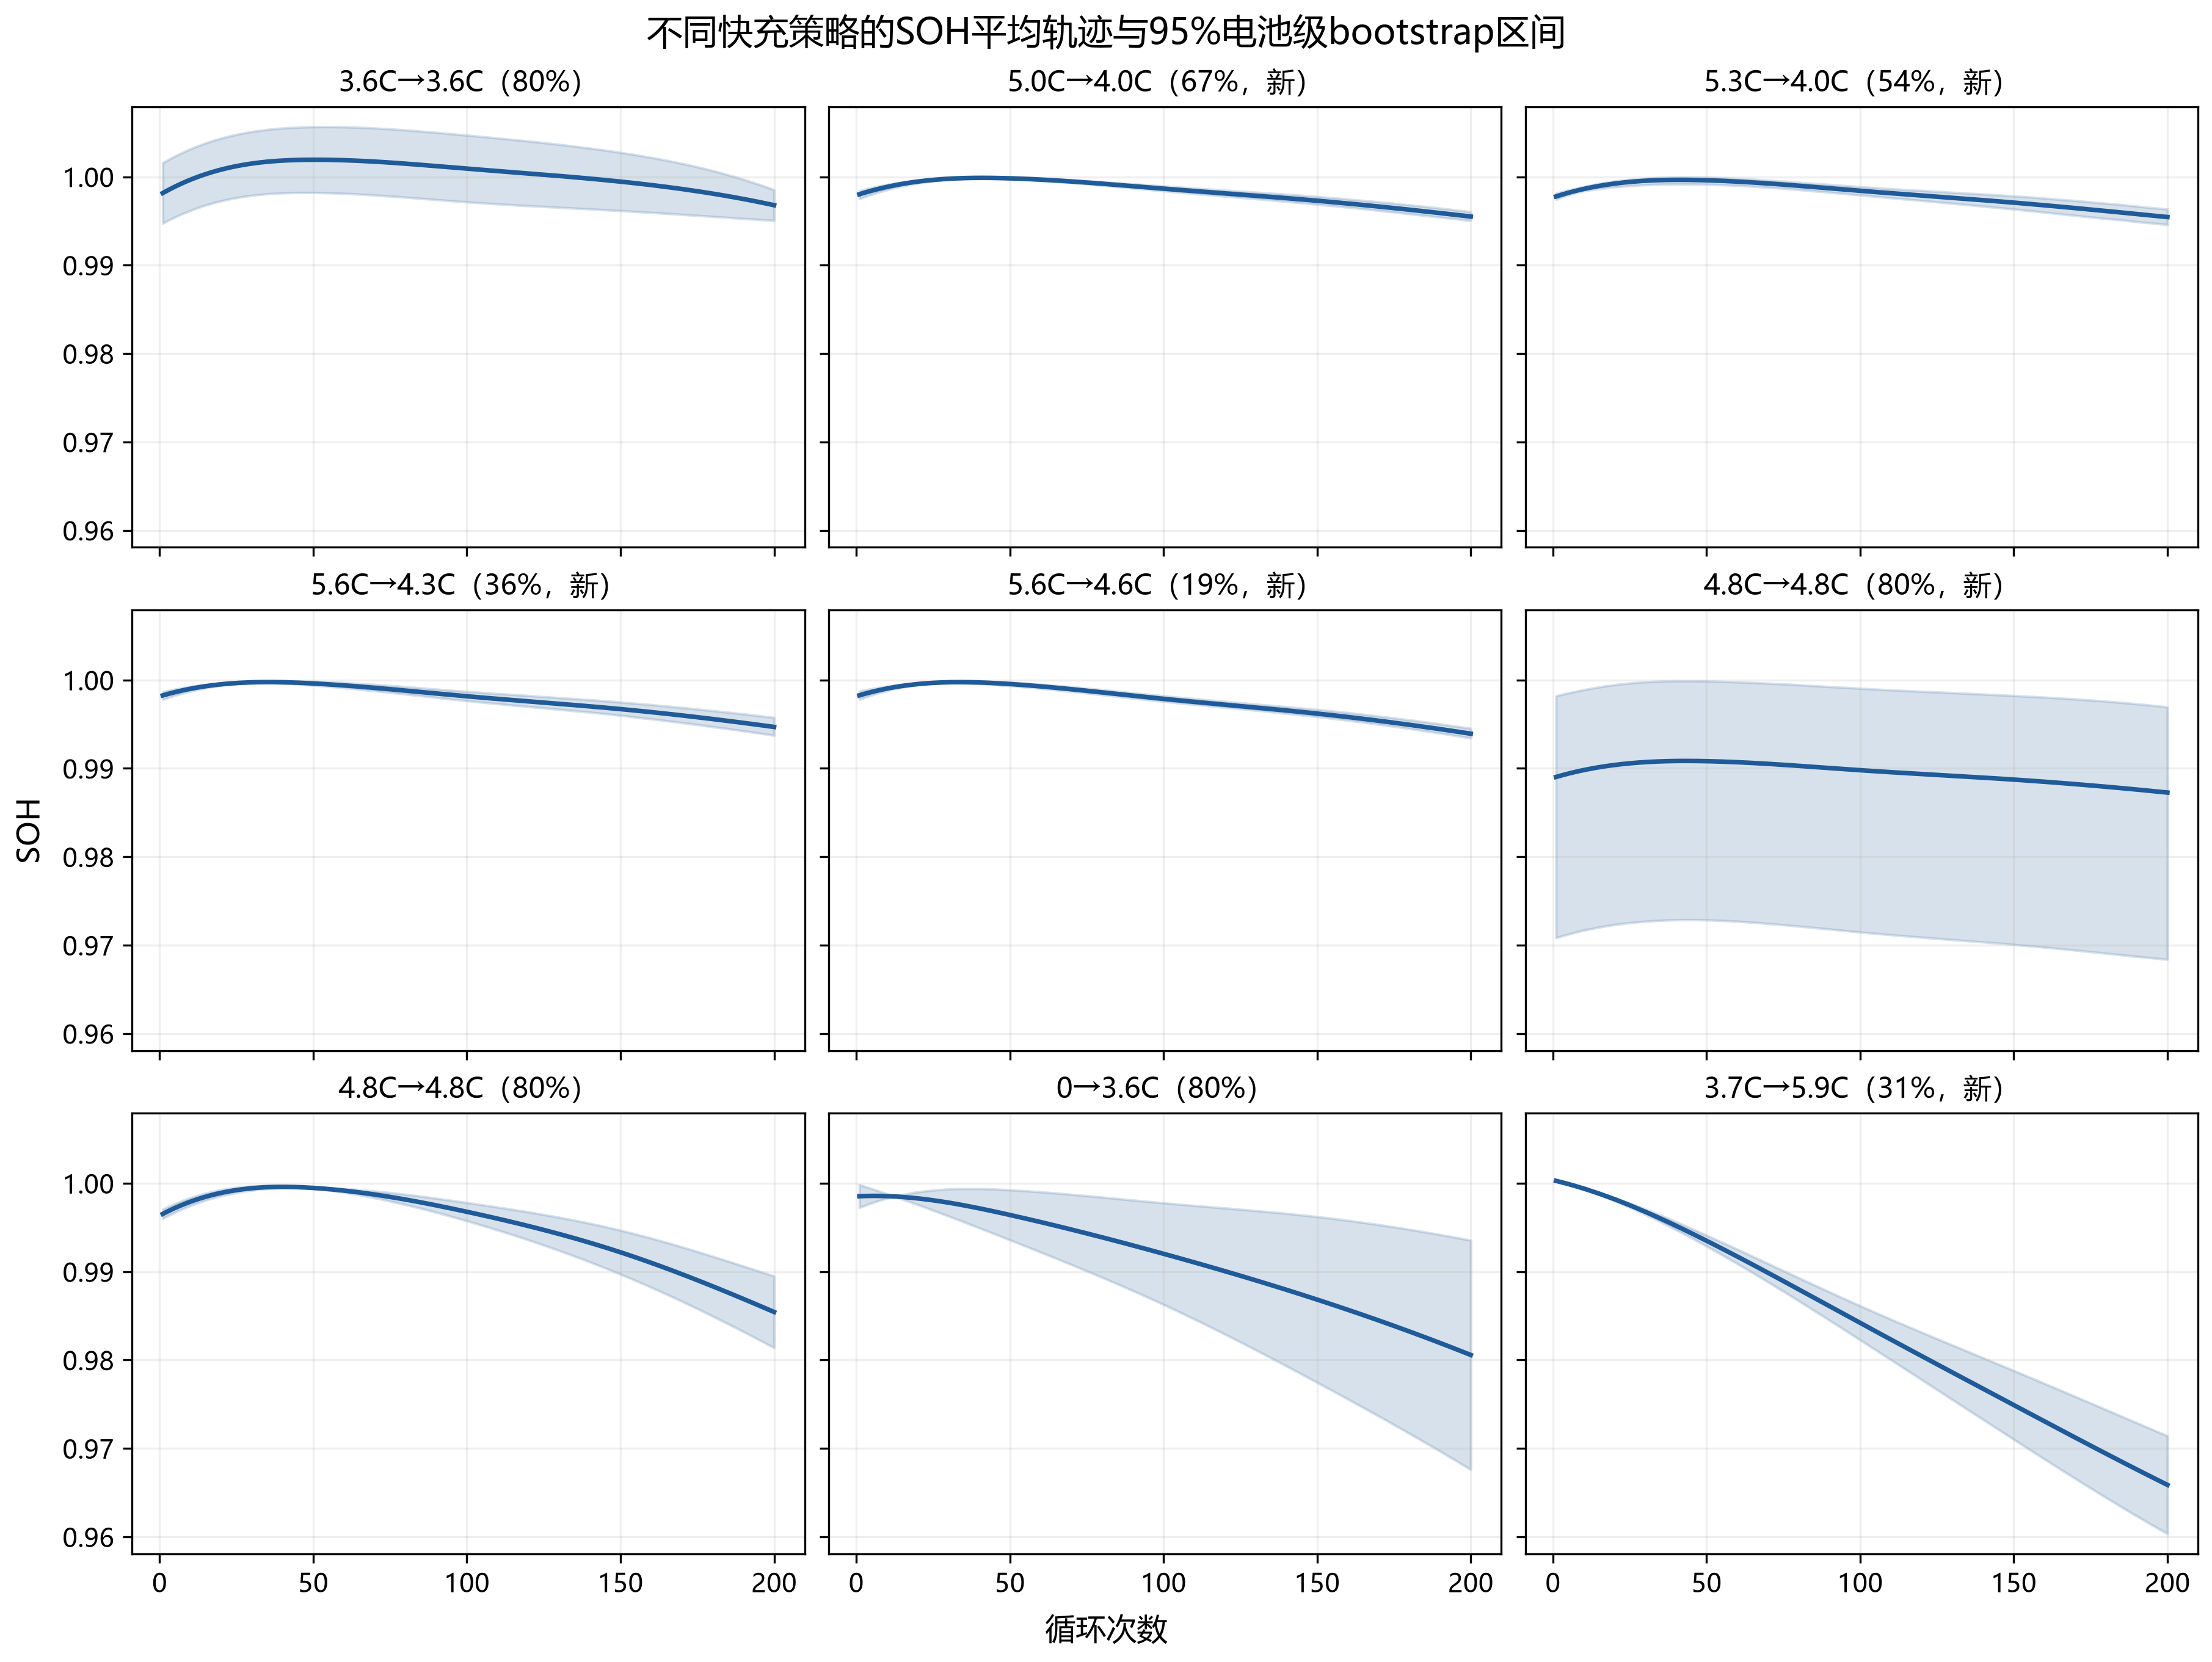
\includegraphics[width=0.95\textwidth]{fig_q1_strategy_soh_curves.png}
\caption{各策略 SOH 曲线（函数型岭主模型拟合）}\label{fig:q1_soh}
\end{figure}

\begin{figure}[H]\centering
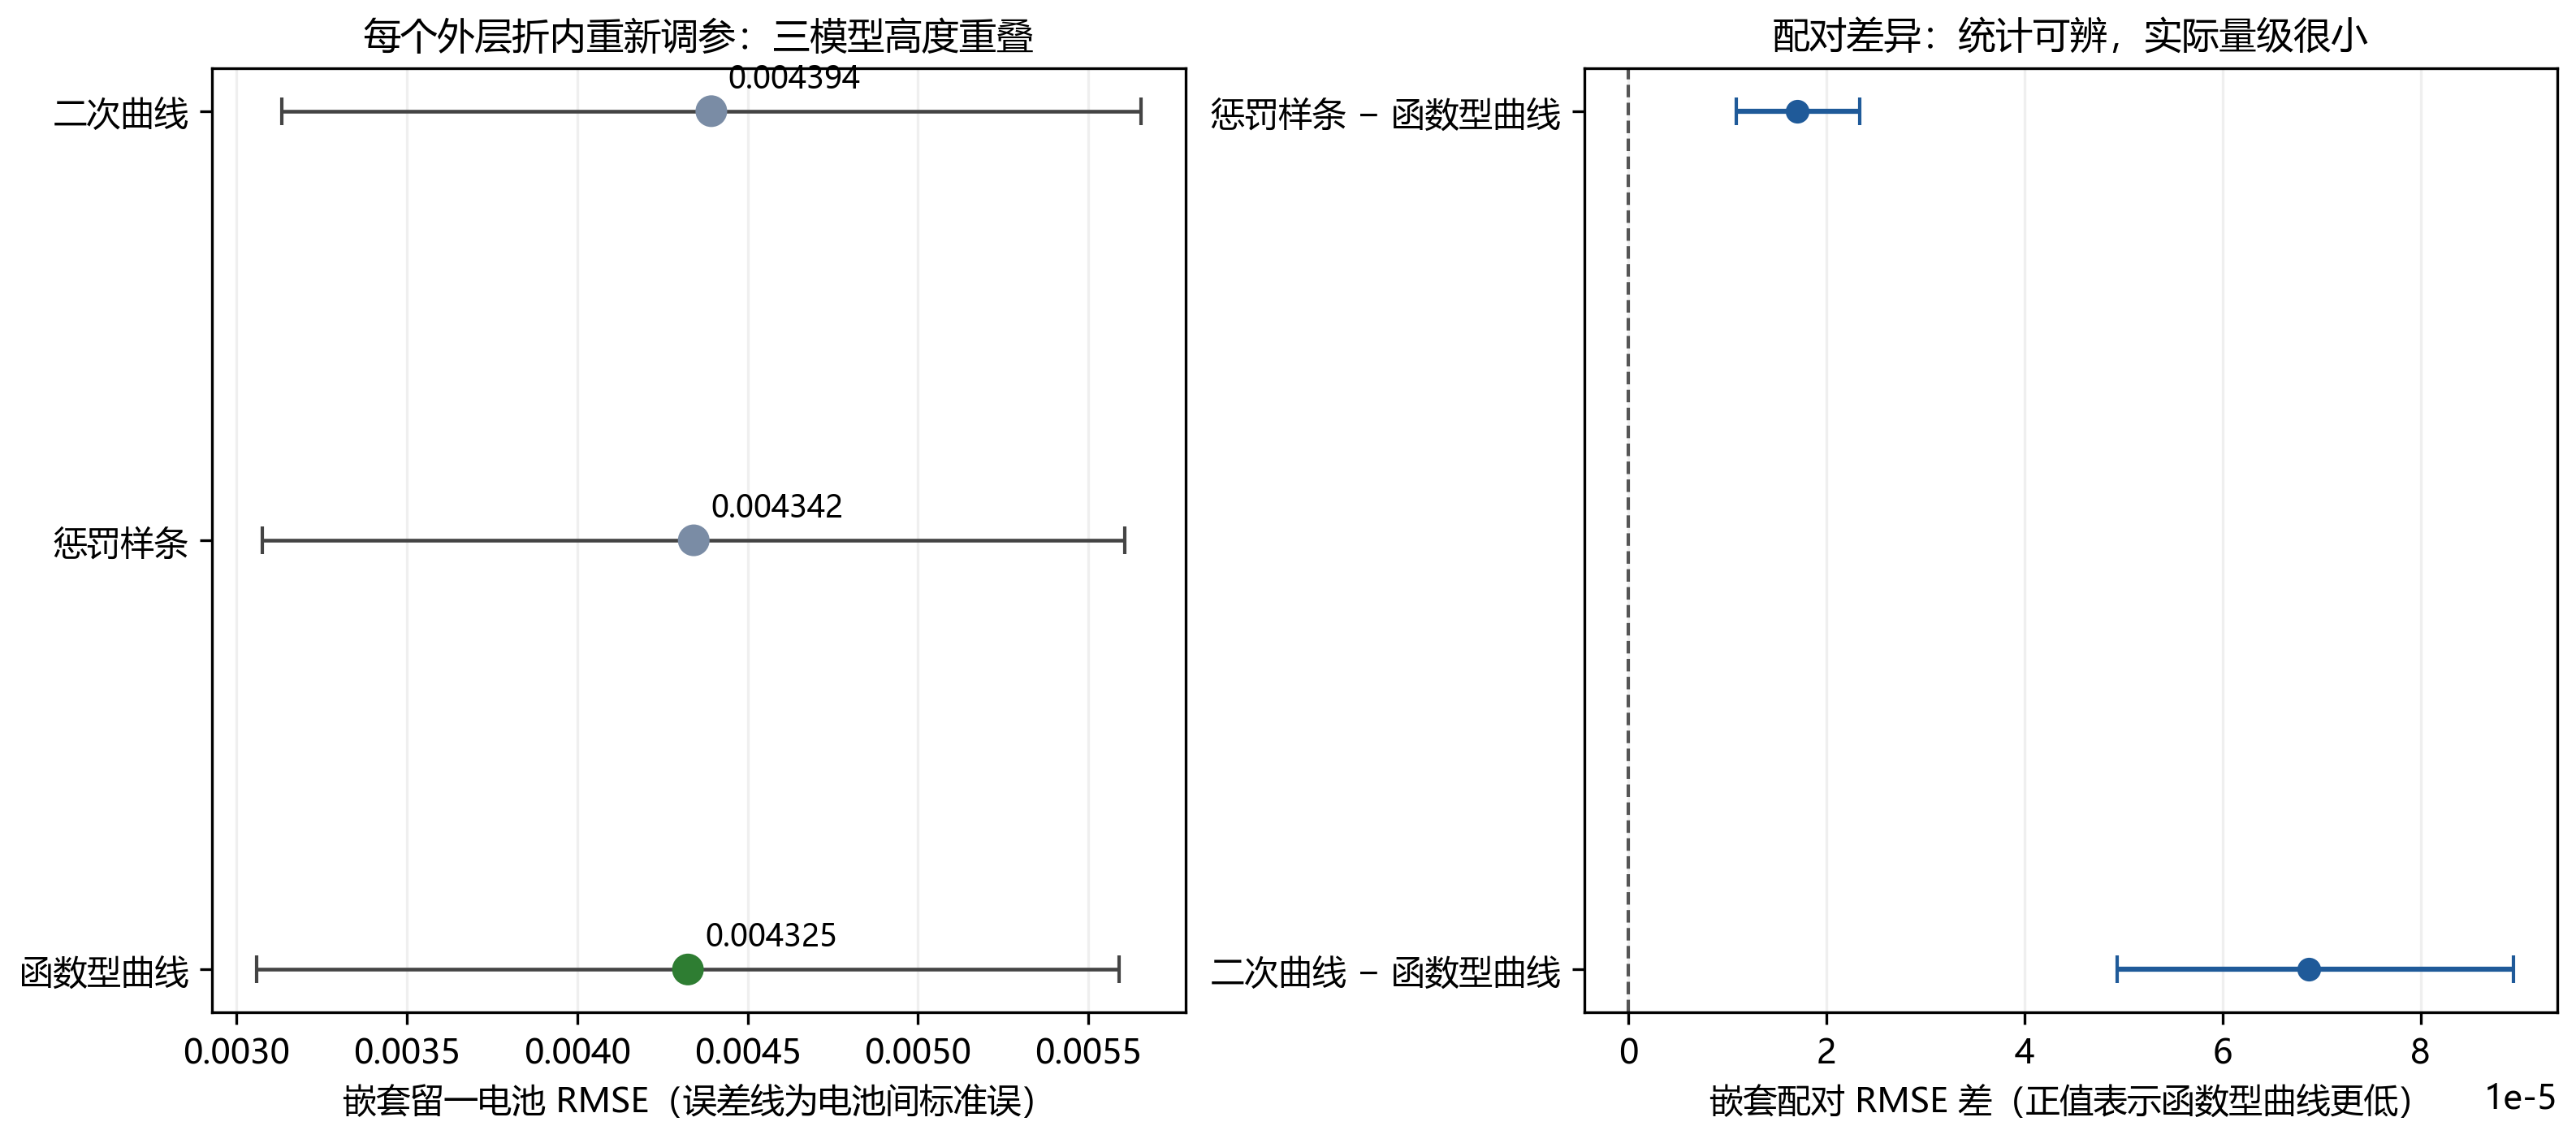
\includegraphics[width=0.9\textwidth]{fig_q1_model_comparison.png}
\caption{三候选模型 LOBO 误差对比}\label{fig:q1_model}
\end{figure}

\subsection{策略寿命分布与典型策略识别}
由于数据无 80\% 终点，以第 200 循环 SOH（SOH200）与前 200 循环 SOH 损失两个指标共同描述寿命表现。9 种策略的完整估计见表 \ref{tab:q1}，SOH200 分布在 $0.9659\sim0.9968$ 之间，极差约 3.1 个百分点。

\begin{table}[H]\centering
\caption{各策略寿命代理指标（按 SOH200 降序）}\label{tab:q1}
\begin{tabular}{clccc}
\toprule
排名 & 策略 & SOH200 & 前200循环损失 & 充电时间/min\\
\midrule
1 & $3\_6C$--$80PER\_3\_6C$ & 0.9968 & 0.0014 & 13.388\\
2 & $5C\_67PER\_4C$（新） & 0.9955 & 0.0025 & 10.159\\
3 & $5\_3C\_54PER\_4C$（新） & 0.9954 & 0.0023 & 10.158\\
4 & $5\_6C\_36PER\_4\_3C$（新） & 0.9947 & 0.0036 & 10.215\\
5 & $5\_6C\_19PER\_4\_6C$（新） & 0.9939 & 0.0043 & 10.250\\
6 & $4\_8C\_80PER\_4\_8C$（新） & 0.9873 & 0.0018 & 11.160\\
7 & $4\_8C\_80PER\_4\_8C$ & 0.9854 & 0.0111 & 13.082\\
8 & $80PER\_3\_6C$ & 0.9806 & 0.0180 & 14.280\\
9 & $3\_7C\_31PER\_5\_9C$（新） & 0.9659 & 0.0344 & 10.852\\
\bottomrule
\end{tabular}
\end{table}

典型长寿命策略为 $3\_6C$--$80PER\_3\_6C$、$5C\_67PER\_4C$ 与 $5\_3C\_54PER\_4C$，三者进入 Top 3 的 bootstrap 概率分别为 $91.4\%$、$85.8\%$ 与 $77.2\%$（前两者达到 80\% 稳定性标准）。典型短寿命策略为 $3\_7C\_31PER\_5\_9C$、$80PER\_3\_6C$ 与 $4\_8C\_80PER\_4\_8C$，进入 Bottom 3 的概率分别为 $100\%$、$81.5\%$ 与 $71.0\%$；其中 $3\_7C\_31PER\_5\_9C$ 的短寿命特征最稳定。

\subsection{两两比较与寿命终点边界}
精确置换检验配合 Holm 校正后，\textbf{36 组 SOH200 两两比较中没有任何策略对显著}——9 种策略每类仅 2--7 块完整电池，两两检验功效有限，故排序仅作为描述性结论，不能反向解释为九种策略完全等效（策略间末段退化率的全局差异由问题二另行检验）。此外，49 块电池均未观测到 80\% SOH 终点，局部线性外推的 $L_{80}$ 只能作为未验证的外推代理，不作为寿命标签。

\subsection{长寿命与短寿命策略的差异解释}
典型长寿命策略的共同特征是\textbf{限制了中高 SOC 区间的充电倍率}：$5C\_67PER\_4C$ 在 67\% SOC 后降至 4C，$5\_3C\_54PER\_4C$ 在 54\% SOC 后降至 4C，$3\_6C$ 则在主要快充区间保持较温和的 3.6C；而典型短寿命策略 $3\_7C\_31PER\_5\_9C$ 在 31\% SOC 即切换至 5.9C，使电池在 31\%--80\% SOC 的较宽区间承受高倍率，其充电时间仅 10.85 min 却对应最低的 SOH200（0.9659）。持续的中高 SOC 高倍率可能增强电化学极化与欧姆发热，增加活性锂损失、界面副反应与析锂风险\upcite{keil2016charging}。

值得注意的是，结果\textbf{不显示"充电时间越长寿命越好"的单调关系}：$5C\_67PER\_4C$ 与 $5\_3C\_54PER\_4C$ 的充电时间约 10.16 min，同时保持较高 SOH200，反而快于更长充电时间但更低 SOH 的 $80PER\_3\_6C$（14.28 min）。这说明\textbf{高倍率出现的 SOC 区间及持续范围，比单一倍率大小或充电时间更能解释策略间寿命差异}，与相同平均倍率下充电协议仍可产生不同寿命的文献观察一致\upcite{zhang2006charging}。此外，$4\_8C\_80PER\_4\_8C$（新结构）受电池 41 初始 SOH 基线影响较大，改用相对 SOH 或排除电池 41 后其排名上升，故不将全部 4.8C 策略归入短寿命组。上述机制解释来自数据关联与电化学文献，不构成独立随机实验下的因果结论。

\section{问题二模型的建立与求解}
\subsection{低维应力坐标}
设 $q=Q_1/100$，两阶段倍率函数为
\begin{equation}
c(s)=\begin{cases}C_1,&0\le s\le q,\\ C_2,&q<s\le0.8,\end{cases}
\end{equation}
据此定义理想恒流充电时间、总电流应力与高 SOC 加权应力：
\begin{equation}
T_0=60\Big(\frac{q}{C_1}+\frac{0.8-q}{C_2}\Big),\quad
J=qC_1+(0.8-q)C_2,\quad
H=\frac12\Big[C_1q^2+C_2(0.8^2-q^2)\Big].
\end{equation}
$J$ 描述主要充电区间的总体倍率暴露，$H$ 对高 SOC 区间赋予更高权重。二者相关系数为 $0.87$，$T_0$ 与 $J$ 相关系数为 $-0.984$，三者不能同时进入正式模型。此外定义"高于阈值 $s_0$ 的 SOC 区间应力"
\begin{equation}
J_{\mathrm{high},s_0}=C_1\max(q-s_0,0)+C_2\big(0.8-\max(q,s_0)\big),\quad s_0\in\{0.5,0.6,0.7\},
\end{equation}
用于隔离中高 SOC 高倍率暴露对退化的作用。

\subsection{约束退化混合模型}
以第 151--200 循环的末段退化率（对数尺度）为响应，建立
\begin{equation}
y_{it}=a_i-r_i x_t-kx_t^2+\varepsilon_{it},\quad x_t=t/200,
\end{equation}
\begin{equation}
\log r_i=\beta_0+\beta_J\widetilde J_{p(i)}+\beta_H\widetilde H_{p(i)}+\beta_S S_{p(i)}+u_i,
\end{equation}
其中 $r_i>0$、$k\ge0$ 保证平均 SOH 单调下降，$u_i$ 为同策略电池差异，$S$ 为"新结构/数据批次"联合标签（不作纯结构因果解释）。模型选择使用留一策略验证、AICc 与系数稳定性。

\subsection{统计显著性}
对策略间末段退化率做全局置换检验：$F=12.50$、置换 $p=5\times10^{-5}$（20000 次置换），表明\textbf{策略标签与末段退化存在全局关联}。在单暴露模型中，高 SOC 应力 $J_{\mathrm{high},70}$（SOC 高于 70\% 区间的倍率暴露）是预测退化最强、方向一致的解释量：其标准化系数为 $0.0039$（对相对损失为正、对 SOH200 为负），单暴露未校正 $p=0.019$；但经四个暴露量的选择校正后 $p=0.065$ 未达显著，且删除极端策略后常数模型胜出（图 \ref{fig:q2_stab}）。因此，$J_{\mathrm{high},70}$ 与退化的关联方向稳健，但\textbf{不能据此宣称 SOC 阈值或参数的独立因果效应}。

\begin{figure}[H]\centering
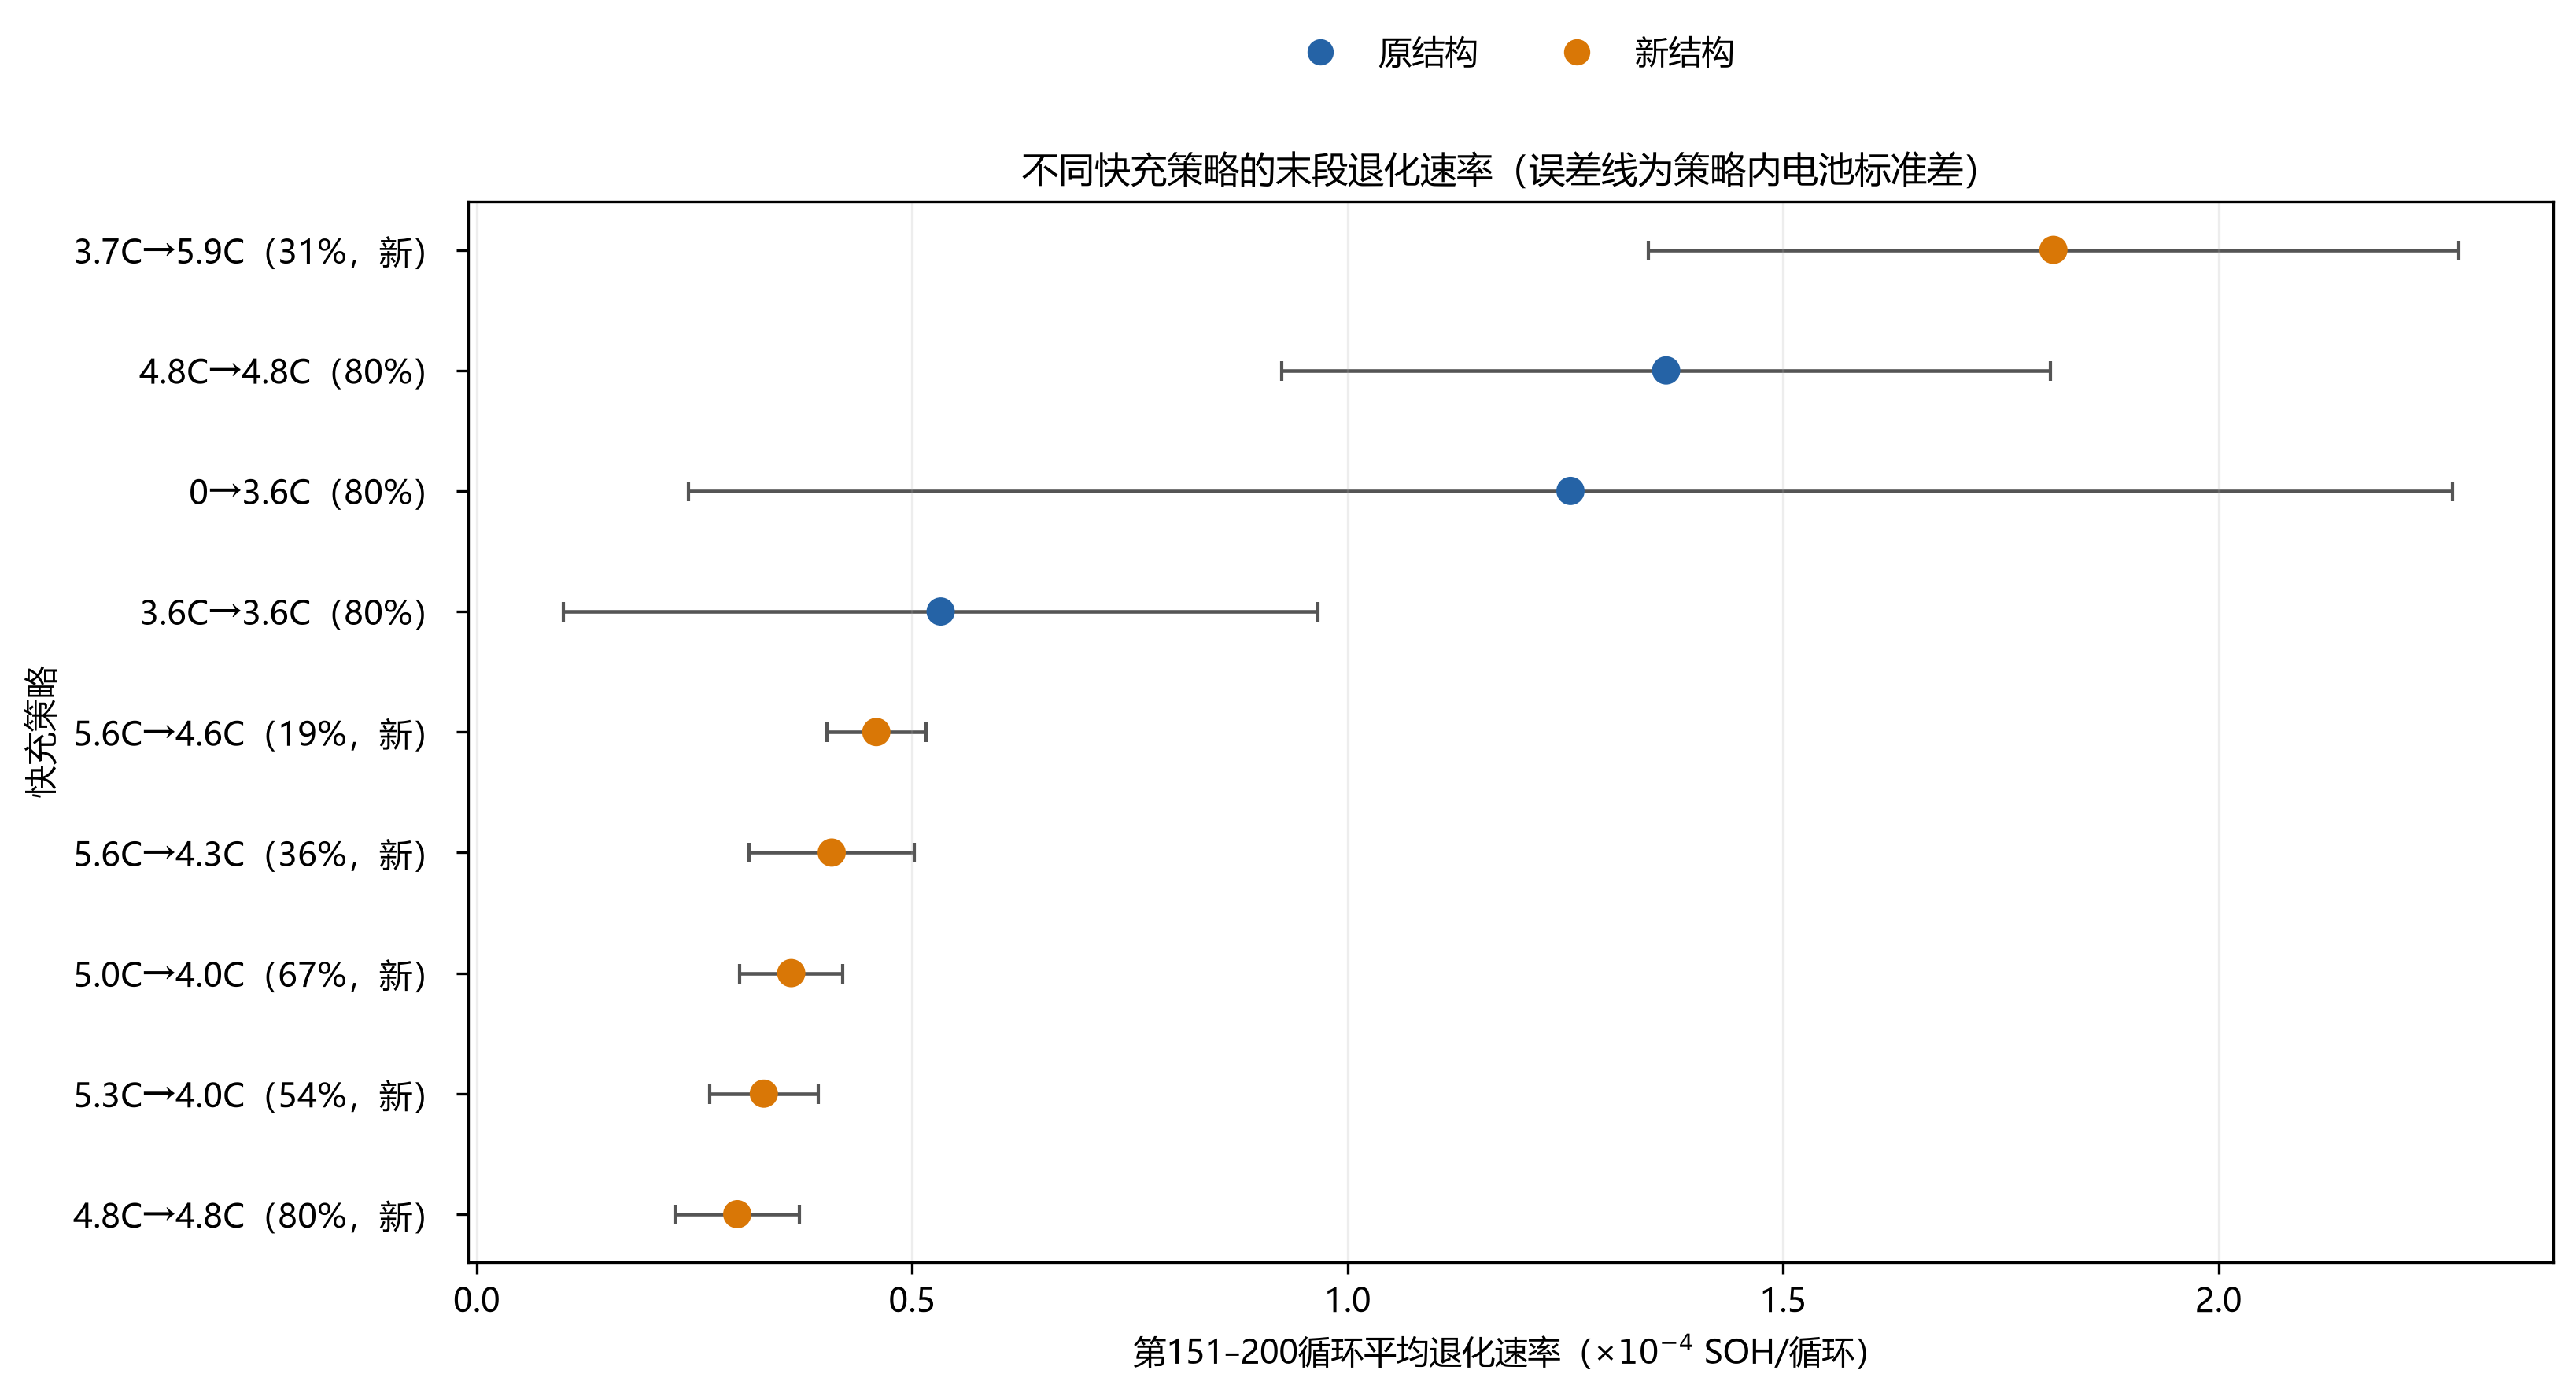
\includegraphics[width=0.9\textwidth]{fig_q2_strategy_late_rate.png}
\caption{各策略末段（151--200 循环）退化率}\label{fig:q2_rate}
\end{figure}

\begin{figure}[H]\centering
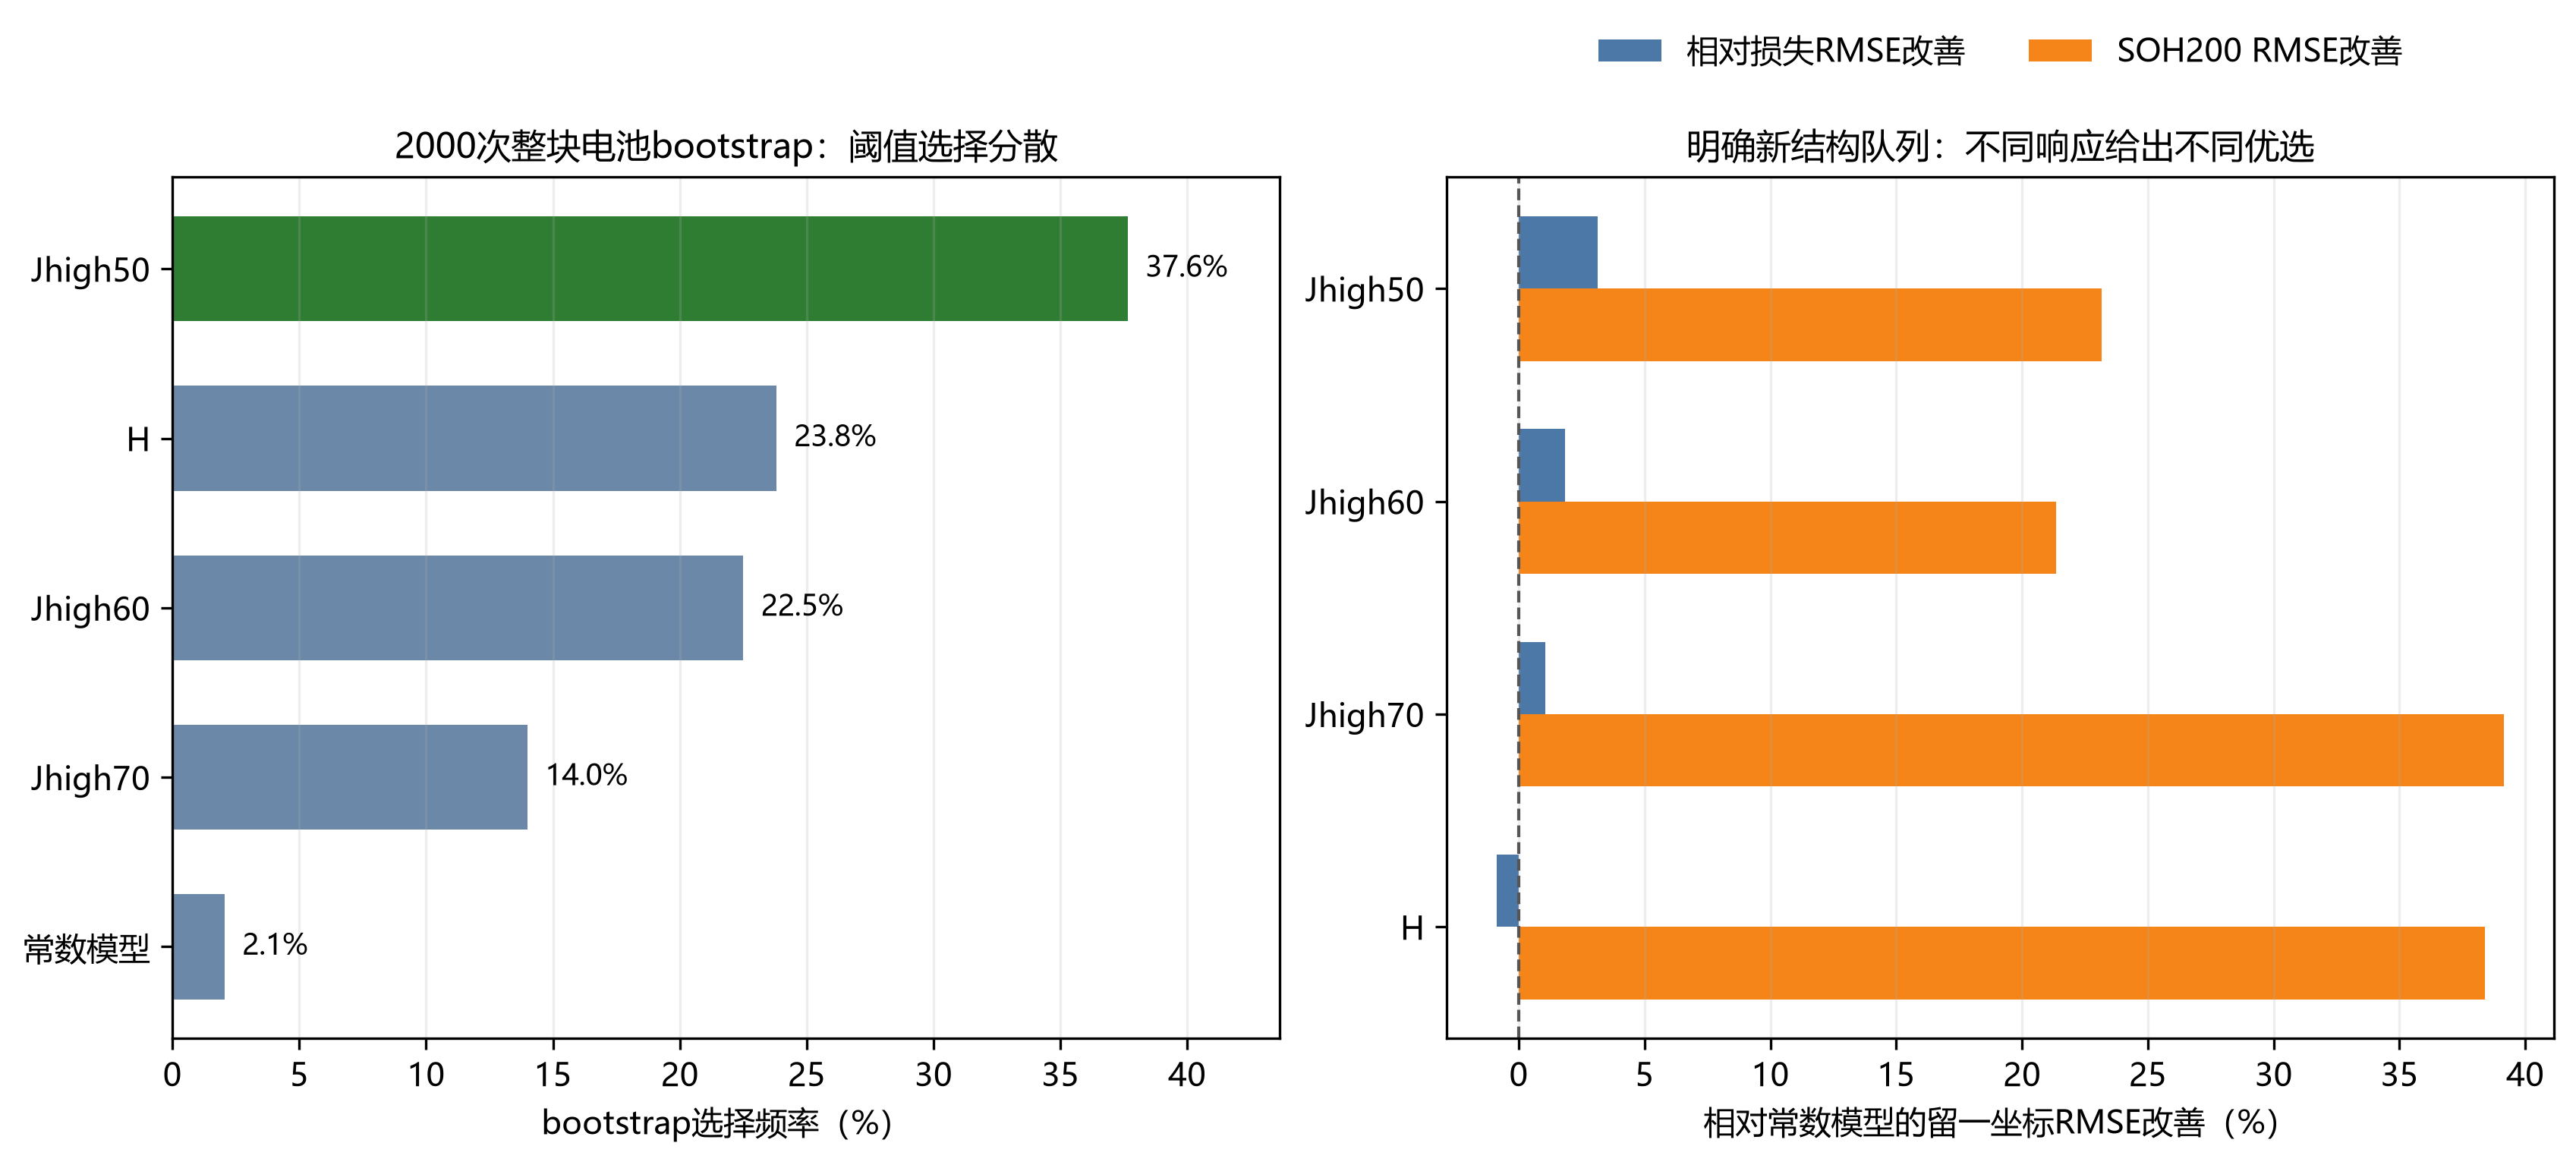
\includegraphics[width=0.9\textwidth]{fig_q2_model_stability.png}
\caption{模型系数稳定性与选择校正}\label{fig:q2_stab}
\end{figure}

\subsection{结构与批次混杂}
两个具有相同 $(4.8,0.8,4.8)$ 参数的策略分属旧/新结构，末段退化率分别为 $0.000137$ 与 $0.000030$，配对置换 $p=0.048$；但结构、数据批次与策略参数完全混杂，无法将此差异干净地归因于"结构"。

\subsection{小问结论}
综上，回答五个小问：\textbf{（1）}策略间末段退化存在全局显著差异；\textbf{（2--3）}$C_1,Q_1,C_2$ 与退化的关联方向一致（高 SOC 高倍率加剧退化），但受稀疏混杂设计限制，不能识别三个参数的独立因果效应；\textbf{（4）}不同 SOC 区间高倍率的差异化作用方向与机理预期一致，但证据强度不足以形成因果断言；\textbf{（5）}结论的机制可解释为高 SOC 下高倍率促进锂析出与极化加剧，其局限性在于设计混杂与样本量不足\upcite{keil2016charging}。

\section{问题三模型的建立与求解}
\subsection{特征提取}
从每块电池前 $L$ 循环的观测提取三类特征（表 \ref{tab:q3feat}）：\textbf{（1）轨迹形态特征}——采样 SOH 点位、全区间线性斜率、多窗口局部斜率、近期曲率（近期斜率与前期斜率之差）、线性拟合残差标准差、近期变化范围；\textbf{（2）运行状态动态特征}——内阻、平均温度、充电时间的均值、近期均值与斜率；\textbf{（3）策略参数与应力坐标}——$C_1,q,C_2$、$C_1$ 缺失标记，以及 $J,H,J_{\mathrm{high},50/60/70}$。特征在每折内部用训练电池的中位数填充缺失、标准化。

\begin{table}[H]\centering
\caption{问题三特征集}\label{tab:q3feat}
\begin{tabular}{ll}
\toprule
类别 & 特征\\
\midrule
轨迹形态 & 采样 SOH 点位、全区间斜率、多窗口局部斜率、曲率、残差标准差、近期范围\\
运行状态 & 内阻/平均温度/充电时间的均值、近期均值、斜率（共 9 维）\\
策略参数 & $C_1,q,C_2$、$C_1$ 缺失标记、$J,H,J_{\mathrm{high},50/60/70}$\\
\bottomrule
\end{tabular}
\end{table}

\subsection{候选模型与主模型机制}
比较六类候选模型，主模型 $C\_ridge$（轨迹岭回归）分三步：\textbf{（1）}用前 $L$ 循环提取前缀特征矩阵 $\bm X$；\textbf{（2）}对训练电池的未来轨迹（相对第 $L$ 循环 SOH 的增量）矩阵 $\bm Y$ 做奇异值分解，取前 $k$ 个主成分作为未来形状基 $\bm B$；\textbf{（3）}对特征 $\bm X$ 与未来得分 $\bm Y\bm B$ 做多输出岭回归
\begin{equation}
\min_{\bm W}\ \lVert \bm X\bm W-\bm Y\bm B\rVert_F^2+\alpha\lVert\bm W\rVert_F^2,
\end{equation}
预测时由 $\hat{\bm Y}=\bar{\bm y}+\bm x_*\bm W\bm B^\top$ 重建未来 SOH 轨迹。折内调参选择 $(k,\alpha)$，外层以 40 块完整电池截断至 $L\in\{50,100,150\}$ 循环做留一电池、嵌套选族。

\subsection{模型选择与预测}
综合多长度后冻结 $C\_ridge$。其固定模型族在 $L=150$ 的策略等权 LOBO RMSE 为 $0.000660$，含调参选族的嵌套流程为 $0.000709$；随早期长度增加误差单调下降（图 \ref{fig:q3_len}）。$L=150$ 消融显示仅用动态特征 RMSE $0.000645$ 优于完整模型，说明策略特征在该窗口不提供增量精度。

\begin{figure}[H]\centering
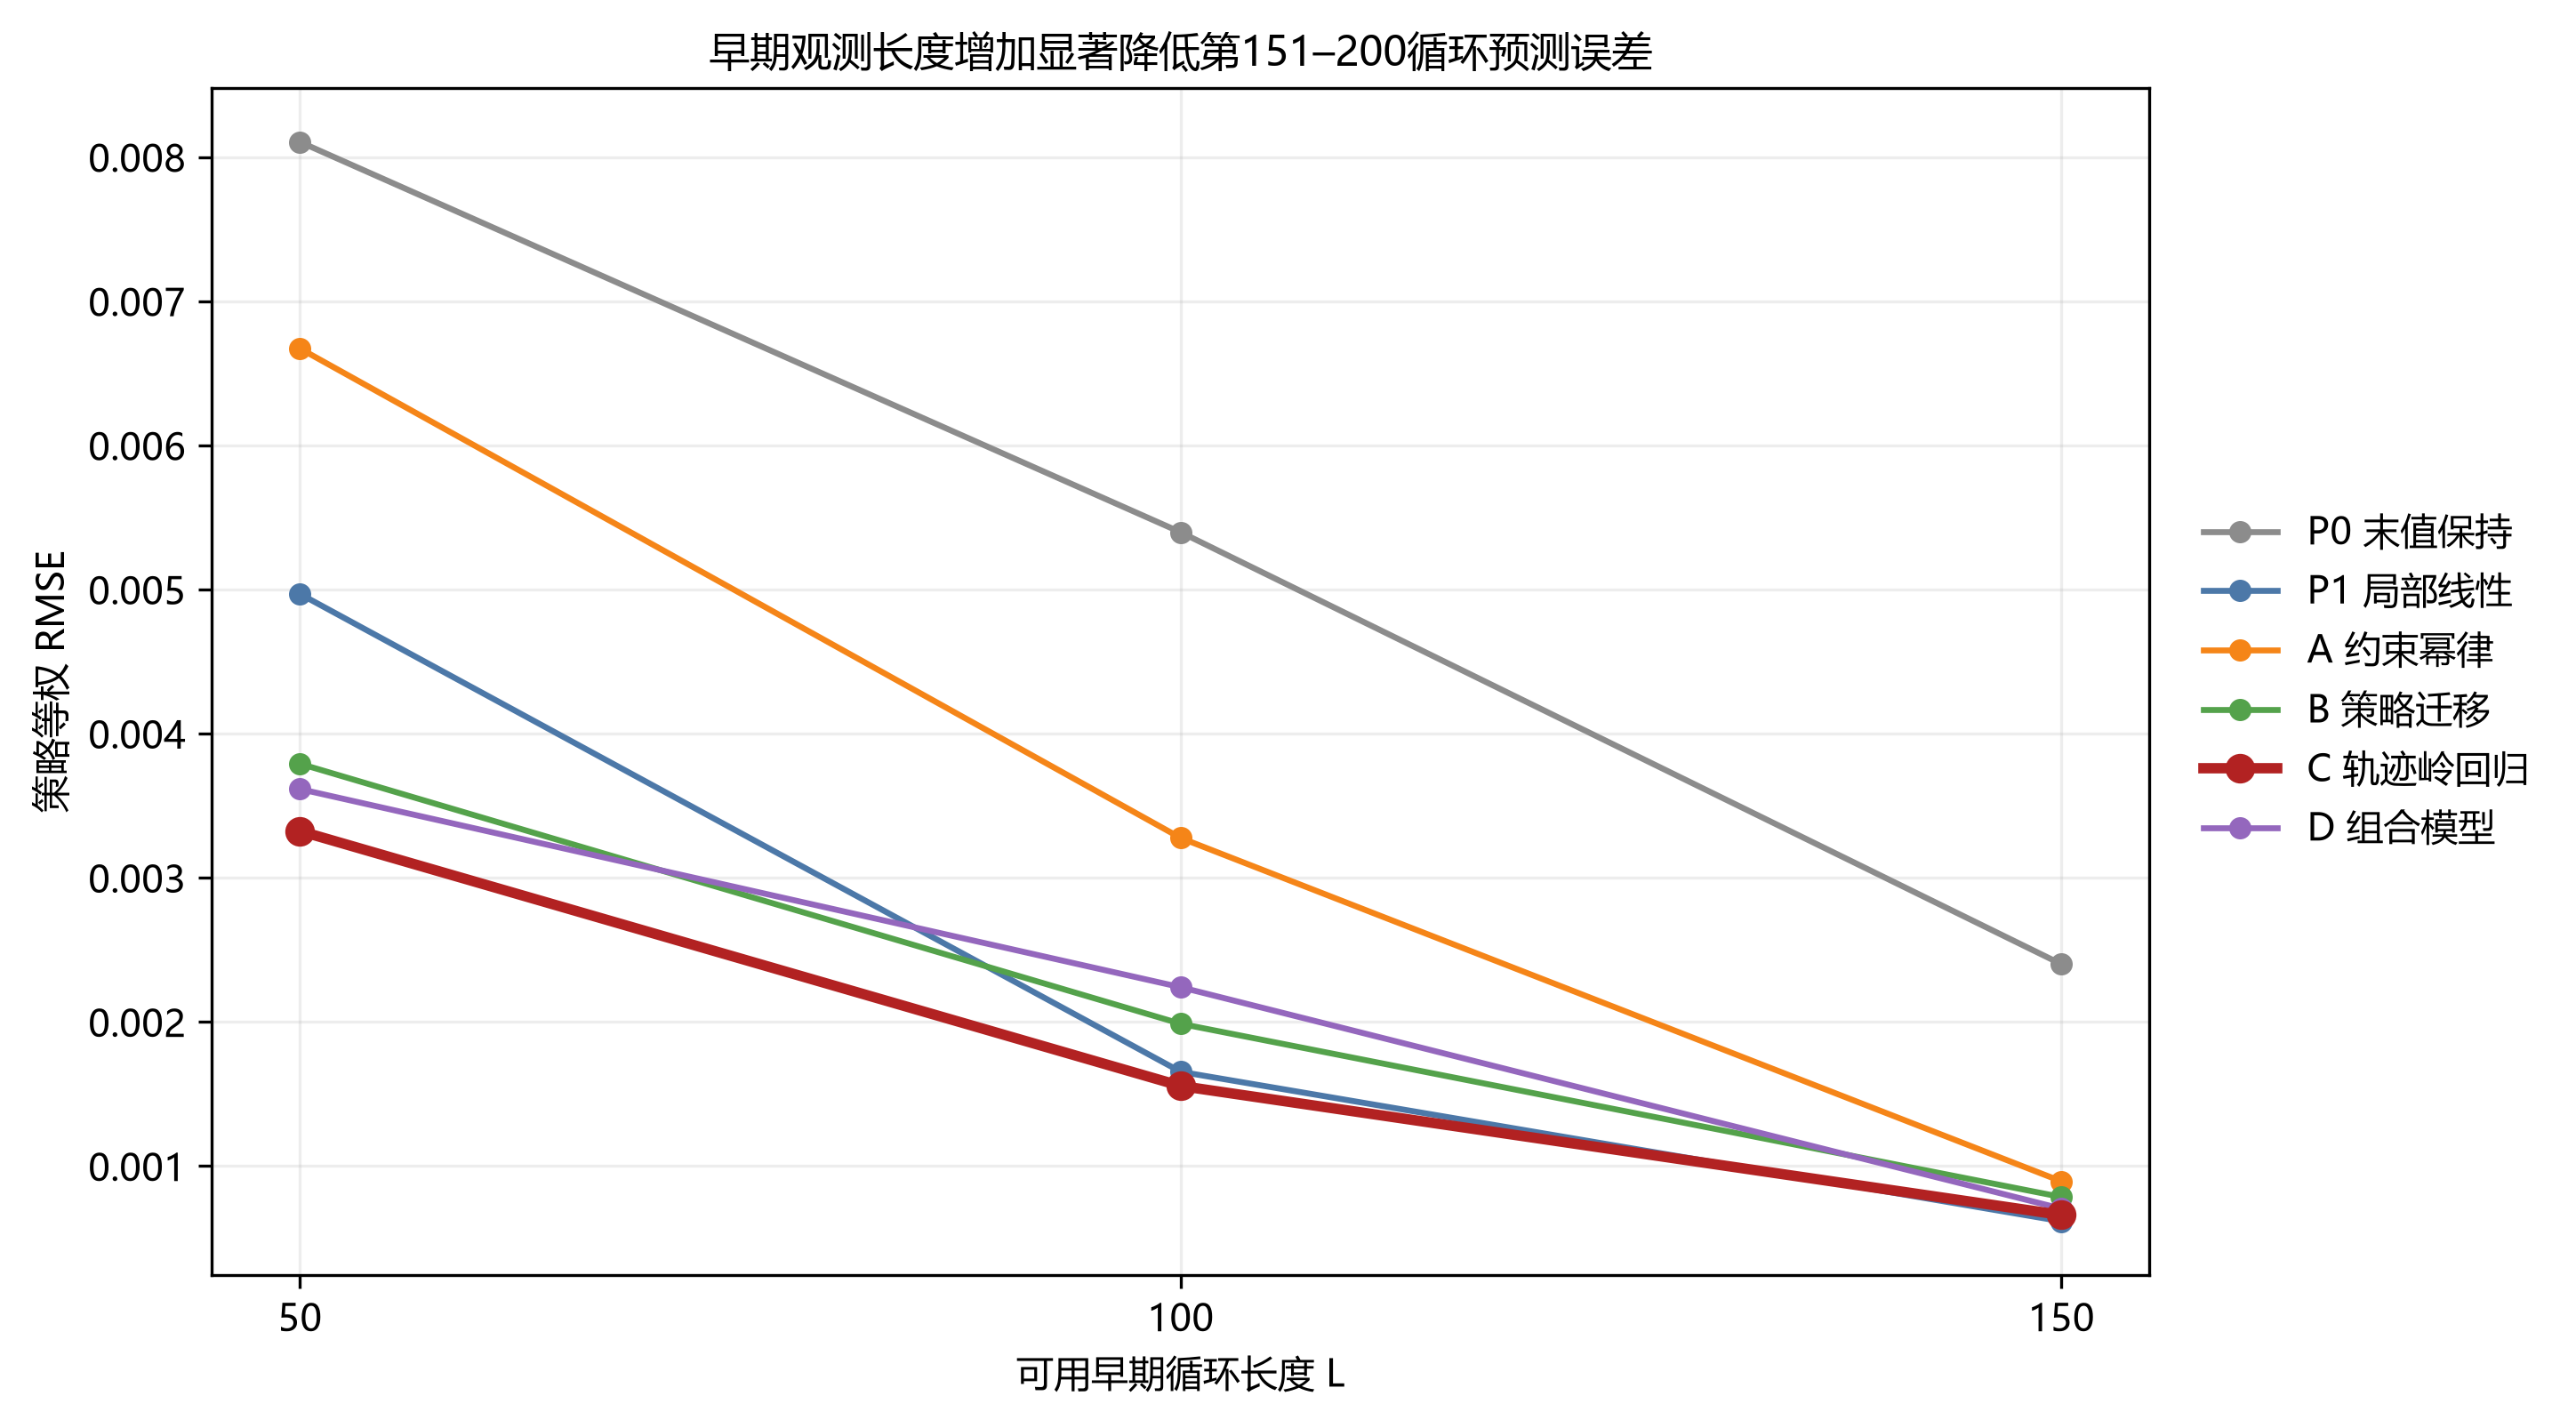
\includegraphics[width=0.85\textwidth]{fig_q3_early_length_rmse.png}
\caption{六候选模型随早期数据长度的 LOBO RMSE}\label{fig:q3_len}
\end{figure}

\begin{figure}[H]\centering
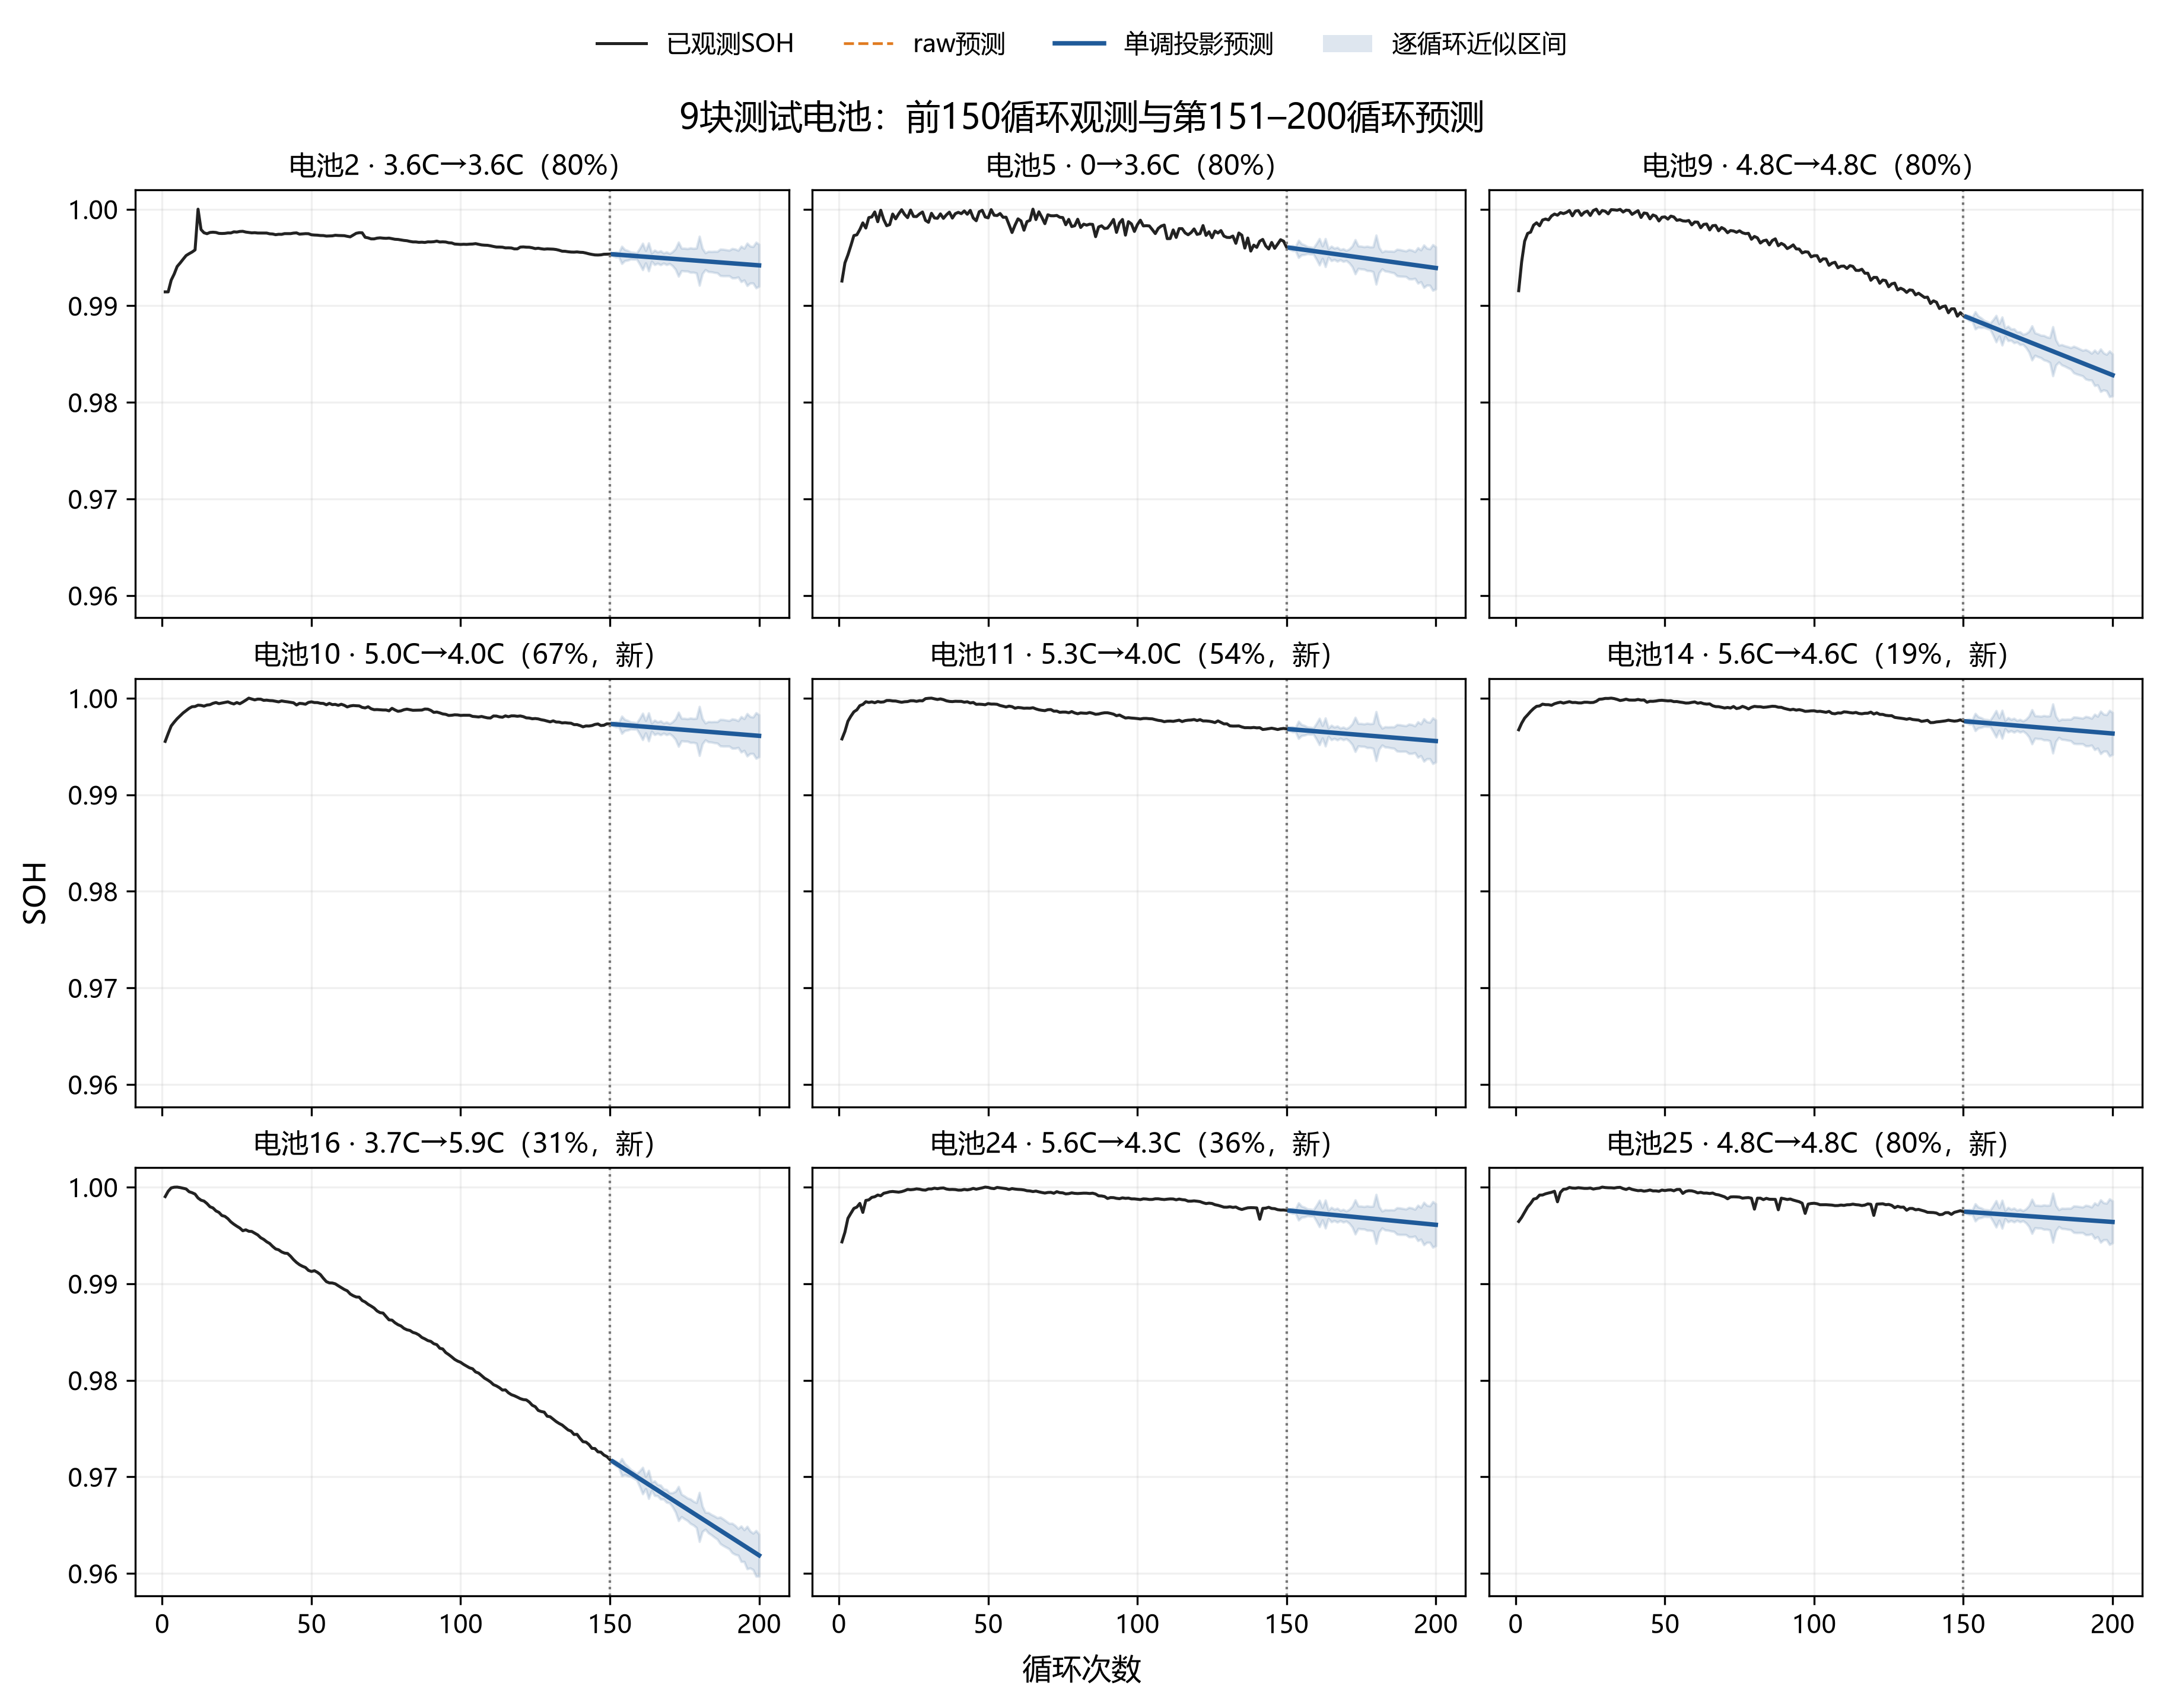
\includegraphics[width=0.95\textwidth]{fig_q3_test_predictions.png}
\caption{9 块测试电池 151--200 循环预测（实线单调投影、阴影保守点区间）}\label{fig:q3_pred}
\end{figure}

\subsection{测试电池预测}
9 块测试电池的预测 SOH200 与保守点区间见表 \ref{tab:q3}。区间由冻结模型族在 40 块训练电池上的外层交叉拟合绝对残差的 97.5\% 经验分位逐循环校准，为偏保守的逐循环点区间，不构成整条轨迹联合区间或独立测试覆盖率。

\begin{table}[H]\centering
\caption{9 块测试电池预测（部分）}\label{tab:q3}
\begin{tabular}{clccc}
\toprule
电池 & 策略 & 预测 SOH200 & 保守点区间 & 默认情景 $T_{80}$\\
\midrule
2 & $3\_6C$--$80PER\_3\_6C$ & 0.993053 & [0.9904, 0.9957] & 774.0\\
10 & $5C\_67PER\_4C$ & 0.995516 & [0.9929, 0.9981] & 1391.1\\
16 & $3\_7C\_31PER\_5\_9C$ & 0.962027 & [0.9594, 0.9647] & 916.1\\
25 & $4\_8C\_80PER\_4\_8C$ & 0.995728 & [0.9931, 0.9984] & 1804.8\\
\bottomrule
\end{tabular}
\end{table}

\subsection{80\% 寿命外推的边界}
80\% 寿命终点（$T_{80}$）对拟合起点与 raw/projected 口径高度敏感（图 \ref{fig:q3_t80}），有限情景值范围为 691.6--3653.0 循环。由于 49 块电池均未观测到 80\% SOH，$T_{80}$ 只能作为模型情景交点，不具有实证寿命精度，论文将其与短期 LOBO 误差分开陈述。

\begin{figure}[H]\centering
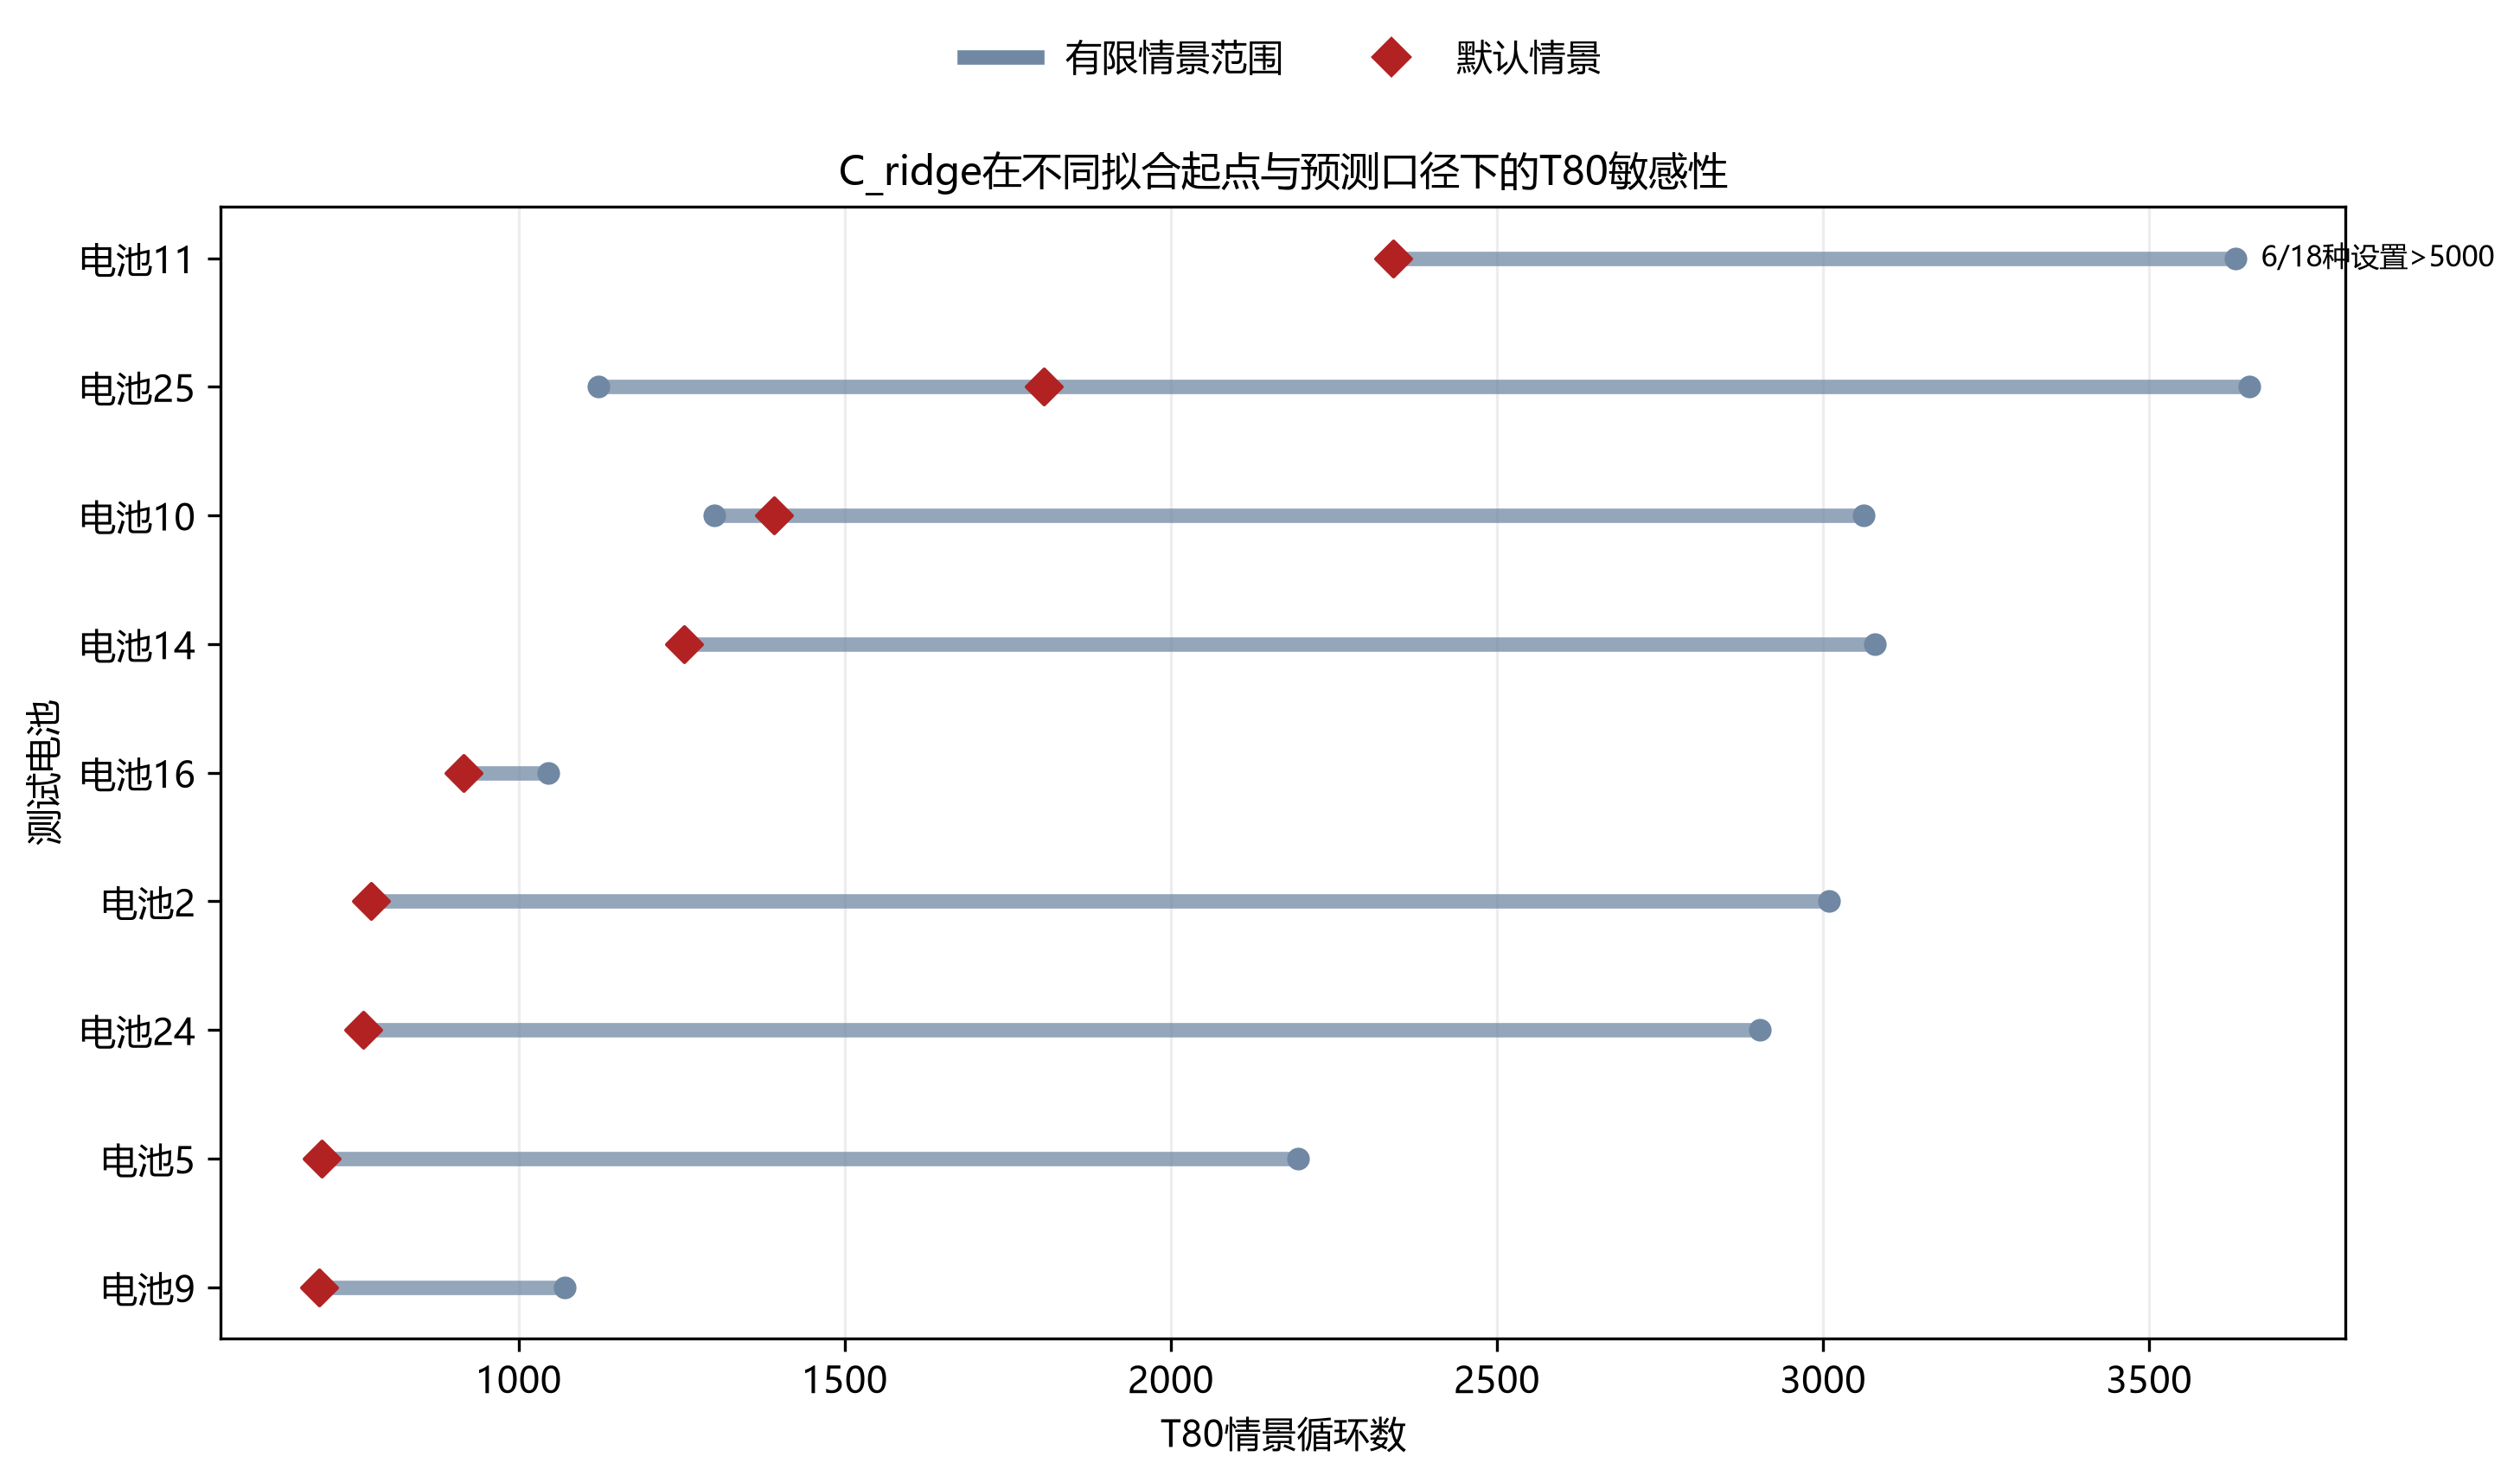
\includegraphics[width=0.85\textwidth]{fig_q3_t80_sensitivity.png}
\caption{$T_{80}$ 情景外推敏感性（红菱形为默认情景）}\label{fig:q3_t80}
\end{figure}

\section{问题四模型的建立与求解}
\subsection{离散 Pareto 主模型（M0）}
对策略 $p$ 定义充电时间与退化量
\begin{equation}
T_p=\operatorname{mean}_{i\in p}(\mathrm{chargetime}_i),\qquad
D_p=\operatorname{mean}_{i\in p}\Big(1-\mathrm{SOH}_{i,200}/b_i\Big),
\end{equation}
其中 $b_i$ 为电池基线容量。若不存在策略 $r$ 使 $T_r\le T_p$ 且 $D_r\le D_p$（至少一项严格），则 $p$ 位于 Pareto 前沿。时间与退化用整块电池 bootstrap 量化不确定性。理论恒流时间 $T_0$ 仅作解释量，实测时间含恒压尾段与结构/批次影响。

\subsection{Pareto 前沿与推荐}
点估计 Pareto 前沿含 3 个策略（表 \ref{tab:q4}），bootstrap 显示前沿成员不稳定。$5\_3C\_54PER\_4C$ 的 Pareto 进入频率最高（0.892），$3\_6C$ 基准为 0.740，$4\_8C$ 新结构为 0.514\allowbreak。

\begin{table}[H]\centering
\caption{点估计 Pareto 前沿（40 块完整电池）}\label{tab:q4}
\begin{tabular}{lccccc}
\toprule
策略 & $n$ & 时间/min & 200 循环退化 & 末段衰减率 & Pareto 频率\\
\midrule
$3\_6C$--$80PER\_3\_6C$ & 2 & 13.382 & 0.000428 & 0.0000500 & 0.740\\
$4\_8C\_80PER\_4\_8C$（新） & 5 & 11.039 & 0.001436 & 0.0000277 & 0.514\\
$5\_3C\_54PER\_4C$ & 7 & 10.043 & 0.001615 & 0.0000315 & 0.892\\
\bottomrule
\end{tabular}
\end{table}

\begin{table}[H]\centering
\caption{推荐策略与典型策略对比}\label{tab:q4c}
\resizebox{\textwidth}{!}{%
\begin{tabular}{lcccc}
\toprule
策略 & 时间/min & 200 循环退化 & 较长寿命时间差 & 较长寿命退化差\\
\midrule
$3\_6C$--$80PER\_3\_6C$（典型长寿命） & 13.382 & 0.000428 & 0 & 0\\
$5\_3C\_54PER\_4C$（推荐） & 10.043 & 0.001615 & $-3.340$ & $+0.001187$\\
$3\_7C\_31PER\_5\_9C$（典型短寿命） & 10.134 & 0.033617 & $-3.249$ & $+0.033189$\\
\bottomrule
\end{tabular}}
\end{table}

\textbf{推荐 $5\_3C\_54PER\_4C$（$C_1=5.3,Q_1=54\%,C_2=4.0$）}：若应用要求优先缩短时间并接受约 0.17\% 的 200 循环相对退化，该策略是近似并列最快组（四个最快新结构策略仅相差不足 0.03 s）中退化最低者。相对典型长寿命策略缩短约 25\% 时间、退化仅增约 0.12 个百分点；相对典型短寿命策略更快 0.09 min 且退化低约 0.032。其机理是低 SOC 段使用较高倍率、较早切换至 4C，形成观测数据支持的时间--退化折中。注意它在时间上仅属于四策略近似并列组，不能宣称显著更快。

\subsection{连续响应面的淘汰（M1）}
受限连续响应面（单 $J$ 岭模型）在 oracle 坐标压力测试中平均 RMSE 为 $0.015827$，相对常数基线改善为 $-0.006806$，7 折中 6 折未优于常数基线，因此\textbf{连续三参数优化被正式淘汰}，正式答案退回离散 Pareto。

\subsection{合理性、适用范围与外推风险}
推荐合理性来自四条证据：位于点估计 Pareto 前沿、bootstrap Pareto 频率最高、两种时间口径下前沿不变、SOH200 与末段斜率方向一致。结论严格限定在 9 个已观测策略范围内，不宣称 $C_1,Q_1,C_2$ 的独立因果最优值，不外推到未观测倍率、SOC 区间或新电芯结构\upcite{keil2016charging,schuster2015nonlinear}。

\section{灵敏度分析}
\subsection{清洗规则敏感性}
固定 3 处修复但改变局部趋势窗口（7/11/15 点）后，策略排序不变；保留异常原始值仅影响个别策略指标。
\subsection{响应口径敏感性}
Q1 以 SOH200、前 200 循环损失、曲线面积与末段斜率多口径检验，策略排序高度一致；Q4 的退化代理允许为负（受基线噪声影响），如 3.6C 策略退化均值为 0.000428、bootstrap 区间下界为 $-0.0015$，已接近测量噪声地板。
\subsection{时间口径敏感性}
Q4 采用 40 块完整电池逐循环充电时间均值为主口径，官方汇总口径作敏感性审计；两口径在部分策略差异明显（如旧结构 4.8C 为 10.45 与 13.08 min），但 Pareto 前沿与权重选择不变。
\subsection{权重敏感性}
Q4 权重扫描中，全 9 策略 min-max 缩放下 $\lambda=0.1\sim1.0$ 选 5.3C；仅 3 个 Pareto 点缩放下 $\lambda=0\sim0.5$ 选 3.6C、$\lambda=0.6\sim1.0$ 选 5.3C，说明膝点依赖标准化集合，故正式结论以 Pareto 与条件约束为主，权重仅描述偏好敏感性。

\section{模型评价与推广}
\subsection{模型优点}
\begin{itemize}
\item 数据清洗最小干预、全程审计留痕，修复决策与人工核对一致；
\item 始终以整块电池为推断单位，正确处理重复测量与聚类重采样；
\item 多模型互证（函数型岭/样条/多项式），并用置换检验、选择校正、bootstrap 量化不确定性；
\item 诚实地报告了设计混杂导致的因果识别边界，不强行宣称参数独立效应。
\end{itemize}
\subsection{模型不足}
\begin{itemize}
\item 9 种策略的稀疏混杂设计使 $C_1,Q_1,C_2$ 独立因果效应不可识别；
\item 无真实 80\% SOH 终点，寿命终点均为外推；
\item 2 电池策略（如 3.6C）的分布组合极少，bootstrap 只能作粗粒度证据。
\end{itemize}
\subsection{推广方向}
可引入层次贝叶斯模型刻画策略总体与电池个体差异并部分汇聚\upcite{jiang2021bayesian,zhou2023bayesian}，在闭环优化框架中结合贝叶斯优化与不确定性进行实验设计\upcite{attia2020closed}，并针对末段斜率反映的退化反转做更细致的机理分析\upcite{schuster2015nonlinear}。

% ============ AI 工具使用声明（须在参考文献之前） ============
\section*{AI 工具使用声明}
本参赛队在竞赛过程中使用了 AI 工具，主要用于【代码调试、语言润色、数据处理与建模方案讨论】，详细使用情况见支撑材料中"AI 工具使用详情.pdf"。核心建模思路、模型选择、结果分析与关键结论均由参赛队独立完成，AI 生成内容已经过逐项人工审查与核实。

% ============ 参考文献 ============
\begin{thebibliography}{99}
\bibitem{severson2019data} Severson K A, Attia P M, Jin N, et al. Data-driven prediction of battery cycle life before capacity degradation[J]. Nature Energy, 2019, 4(5): 383-391.
\bibitem{attia2020closed} Attia P M, Grover A, Jin N, et al. Closed-loop optimization of fast-charging protocols for batteries with machine learning[J]. Nature, 2020, 578(7795): 397-402.
\bibitem{jiang2021bayesian} Jiang B, Gent W E, Mohr F, et al. Bayesian learning for rapid prediction of lithium-ion battery-cycling protocols[J]. Joule, 2021, 5(12): 3187-3203.
\bibitem{keil2016charging} Keil P, Jossen A. Charging protocols for lithium-ion batteries and their impact on cycle life[J]. Journal of Energy Storage, 2016, 6: 125-141.
\bibitem{schuster2015nonlinear} Schuster S F, Bach T C, Fleder E, et al. Nonlinear aging characteristics of lithium-ion cells under different operational conditions[J]. Journal of Energy Storage, 2015, 1: 44-53.
\bibitem{saxena2019accelerated} Saxena S, Xing Y, Kwon D, et al. Accelerated degradation model for C-rate loading of lithium-ion batteries[J]. International Journal of Electrical Power \& Energy Systems, 2019, 107: 438-445.
\bibitem{richardson2017gaussian} Richardson R R, Osborne M A, Howey D A. Gaussian process regression for forecasting battery state of health[J]. Journal of Power Sources, 2017, 357: 209-219.
\bibitem{liu2019modified} Liu K, Hu X, Wei Z, et al. Modified Gaussian process regression models for cyclic capacity prediction of lithium-ion batteries[J]. IEEE Transactions on Transportation Electrification, 2019, 5(4): 1225-1236.
\bibitem{zhou2023bayesian} Zhou Z, Howey D A. Bayesian hierarchical modelling for battery lifetime early prediction[J]. IFAC-PapersOnLine, 2023, 56(2): 6117-6123.
\bibitem{geslin2023features} Geslin A, van Vlijmen B, Cui X, et al. Selecting the appropriate features in battery lifetime predictions[J]. Joule, 2023, 7(9): 1956-1965.
\bibitem{zhang2006charging} Zhang S S. The effect of the charging protocol on the cycle life of a Li-ion battery[J]. Journal of Power Sources, 2006, 161(2): 1385-1391.
\end{thebibliography}

% ============ 附录 ============
\begin{appendices}
\section{支撑材料文件列表}
\begin{longtable}{lll}
\caption{支撑材料文件列表}\label{tab:files} \\
\toprule
类别 & 路径 & 说明\\
\midrule
数据 & data/processed/q1\_cleaned/*.csv & 清洗后摘要表与循环表\\
结果 & result/q1/paper/*.csv & 问题一结果与结论\\
结果 & result/q2/03\_formal\_validation/ & 问题二正式验证\\
结果 & result/q3/03\_final\_predictions/ & 问题三最终预测\\
结果 & result/q4/02\_full\_validation/ & 问题四全量验证与推荐\\
代码 & src/q1\_models/ 等 & 各问模型核心源码\\
代码 & scripts/q1--q4/ & 各问实验入口脚本\\
\bottomrule
\end{longtable}

\section{核心算法代码}
以下为核心模型源码（完整可运行代码见支撑材料，运行顺序见各 scripts 入口）。
\lstinputlisting{code/q1_core.py}
\lstinputlisting{code/q2_core.py}
\lstinputlisting{code/q3_core.py}
\lstinputlisting{code/q4_core.py}

\section{AI 工具使用详情}
本参赛队在竞赛中使用 AI 工具辅助完成以下环节：
\begin{enumerate}
\item 代码调试与运行环境配置；
\item 语言润色；
\item 数据处理与建模方案讨论。
\end{enumerate}
核心建模思路、模型选择、数值结果核验与最终结论均由参赛队独立完成，AI 生成的代码与文字均已逐项人工审查与核实。详细交互过程见支撑材料"AI 工具使用详情.pdf"。

\end{appendices}

\end{document}
